
\begin{comment}
\begin{figure}[t]
\centering
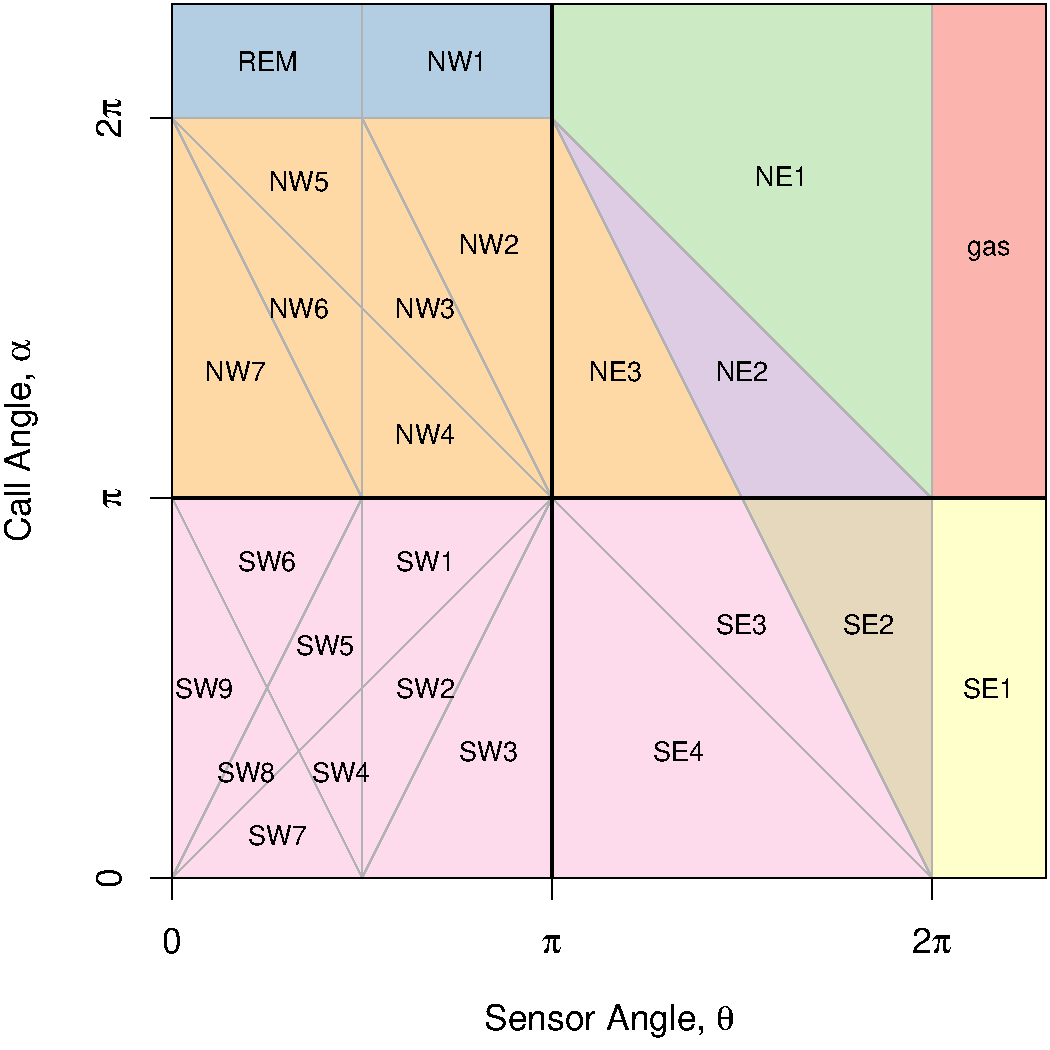
\includegraphics[width=0.6\textwidth]{imgs/equalRegions.pdf}
\caption[REM Model numbers]{The independently derived models for the whole of parameter space. Regions whose solution for $p$ are equal are coloured similarly. Models are numbered by their row, column and then numbered within that area. The models for $\alpha = 2\pi$ or $\theta =  2\pi$ are shown by extending these regions outside of their real boundaries.}
\label{f:equalRegions}
\end{figure}

\end{comment}



%Figure \ref{f:equalRegions} shows the different regions with the upper right being the gas model as derived above and REM being the model from \citep{rowcliffe2008estimating}. Parameter space is broadly split into three rows ($\alpha \le \pi, \pi \le \alpha < 2\pi$ and $\alpha = 2\pi$) and four columns $(\theta \le \pi/2,  \pi/2 \le \theta \le \pi,  \pi \le \theta < 2\pi$ and $\theta = 2\pi$.) Rows and columns define cells. The equation for $p$ in each region is denoted by three numbers referring to rows, columns and region within that cell (see Fig.~\ref{f:equalRegions}).



\subsection{Gas model} \label{gas}

Following \cite{yapp1956theory}, we derive the gas model where sensors can capture animals in any direction and animal's signal is detectable from any direction($ \theta =  2\pi$ and $ \alpha =  2\pi$). We assume that animals are in a homogeneous environment, and move in straight lines of random direction with velocity $v$. We allow that our stationary sensor can capture animals at a detection distance $r$ and that if an animal moves within this detection zone they are captured with a probability of one, while animals outside the zone are never captured.

In order to derive animal density, we need to consider relative velocity from the reference frame of the animals. Conceptually, this requires us to imagine that all animals are stationary and randomly distributed in space, while the sensor moves with velocity $v$. If we calculate the area covered by the sensor during the survey period we can estimate the number of animals the sensor should capture. As a circle moving across a plane, the area covered by the sensor per unit time is $2rv$. The number of expected captures, $z$, for a survey period of $t$, with an animal density of $D$ is $z = 2rvtD$. To estimate the density, we rearrange to get $D = z/2rvt$.

\subsubsection{gREM derivations for different detection and signal widths}
Different combinations of $\theta$ and $\alpha$ would be expected to occur (e.g., sensors have different detection widths and animals have different signal widths). For different combinations $\theta$ and $\alpha$, the area covered per unit time is no longer given by $2rv$. Instead of the size of the sensor detection zone having a diameter of $2r$, the size changes with the approach angle between the sensor and the animal. For any given signal width and detector width and depending on the angle that the animal approaches the sensor, the width of the area within which an animal can be detected is called the profile, $p$. The size of the profile (averaged across all approach angles) is defined as the average profile $\bar{p}$. However, different combinations of $\theta$ and $\alpha$ need different equations to calculate $\bar{p}$. 

We have identified the parameter space for the combinations of $\theta$ and $\alpha$ for which the derivation of the equations are the same (defined as sub-models in the gREM) (Fig.~\ref{f:equalRegions}). For example, the gas model becomes the simplest gREM sub-model (upper right in (Fig.~\ref{f:equalRegions}) and the REM from \citep{rowcliffe2008estimating} is another gREM sub-model where $\theta<\pi/2$ and $\alpha = 2\pi$.

For different values of $\theta$ and $\alpha$, the only thing that changes is that the area covered per unit time is no longer given by $2rv$. Instead of the sensor having a diameter of $2r$, the sensor has a complex diameter that changes with approach angle. The rest of the derivation is just calculating this value for all values of $\alpha$ and $\theta$. However, different regions of this two dimensional parameter space have noncontinuously different models, with different derivations. Therefore we have to identify the regions for which the derivation is the same, and then separately derive $p$ for each region. The separate regions are shown in Fig.~\ref{f:equalRegions}.

\begin{figure}[t]
\centering
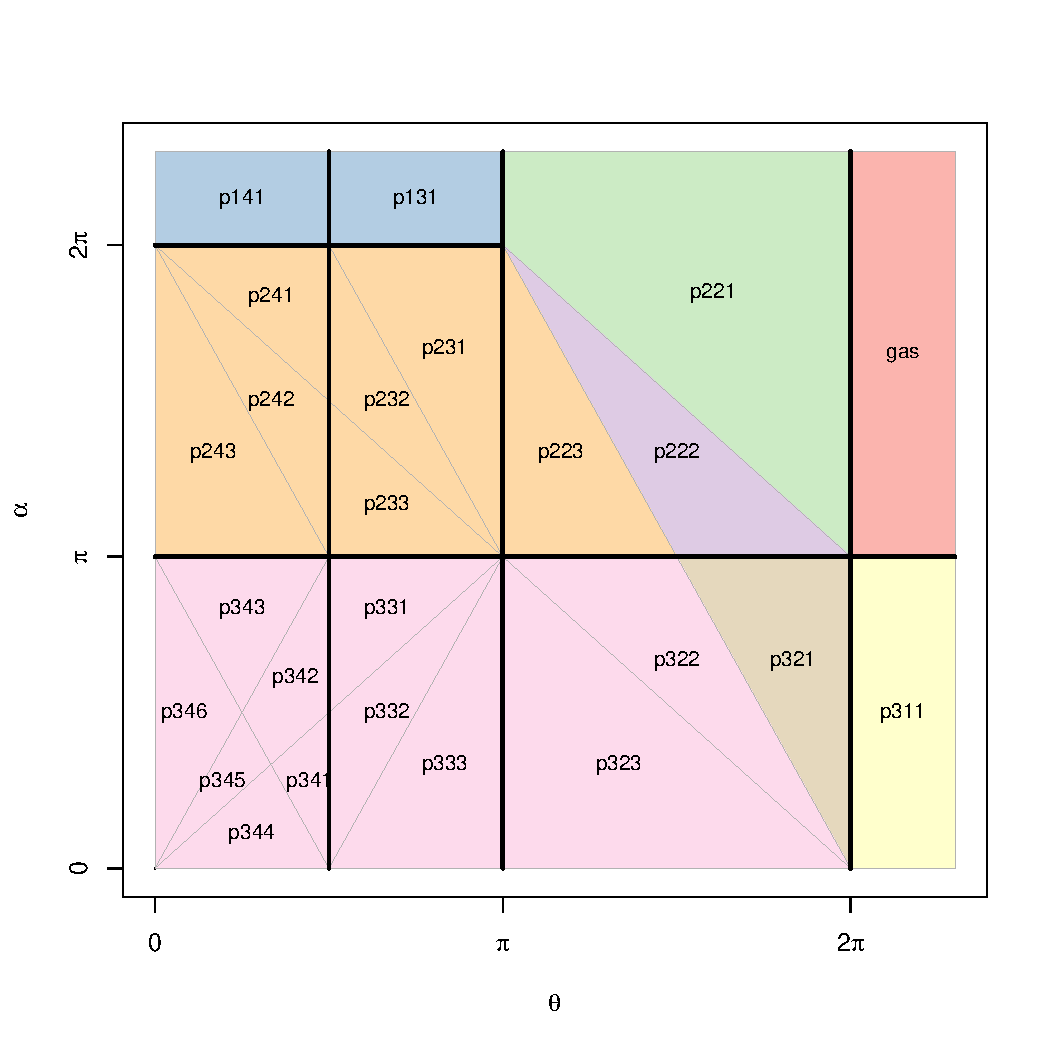
\includegraphics[width=0.6\textwidth]{../imgs/equalRegions.pdf}

\caption{The location of each model in parameter space. Each named model must be derived separately. However, the results of the different models are often the same; areas coloured the same have the same result. Other than the gas model and the REM model, individual models are named after the compass point of the quadrant they are in. The region extends past $\alpha, \theta=2\pi$ to clearly display the models that are defined for only $\alpha=2\pi$ or $\theta=2\pi$ (e.g. the REM model is only definied for $\alpha=2\pi$.}
\label{f:equalRegions}
\end{figure}


\subsection{Model SE1} \label{SE1}

SE1 is very similar to the gas model except that because $\alpha \le \pi$ the profile width is no longer $2r$ but is instead limited by the width of the animal call. We therefore get a profile width of $2r\sin(\alpha/2)$ instead.

\begin{align}
    \bar{p}_{\text{\tiny{SE1}}} =&\frac{1}{\pi} \int\limits_{\frac{\pi}{2}}^{\frac{3 \pi}{2}}2 r \sin{\left (\frac{\alpha}{2} \right )}\;\mathrm{d}x_{1}\label{pSE1Def}\\
    \bar{p}_{\text{\tiny{SE1}}}  =& 2 r \sin{\left (\frac{\alpha}{2} \right )}\label{pSE1Sln}
\end{align}

\subsection{Model NE} \label{NE}

When the detection zone is not a circle, we have more complex profiles  and need to explicitly write functions for the width of the profile for every approach angle. We then use these functions to find the average profile width $\bar{p}$ for all approach angles by integrating across all $2\pi$ angles of approach and dividing by $2\pi$. 



\begin{figure}[t]
        \centering
        \begin{subfigure}[t]{0.34\textwidth}
                \centering
        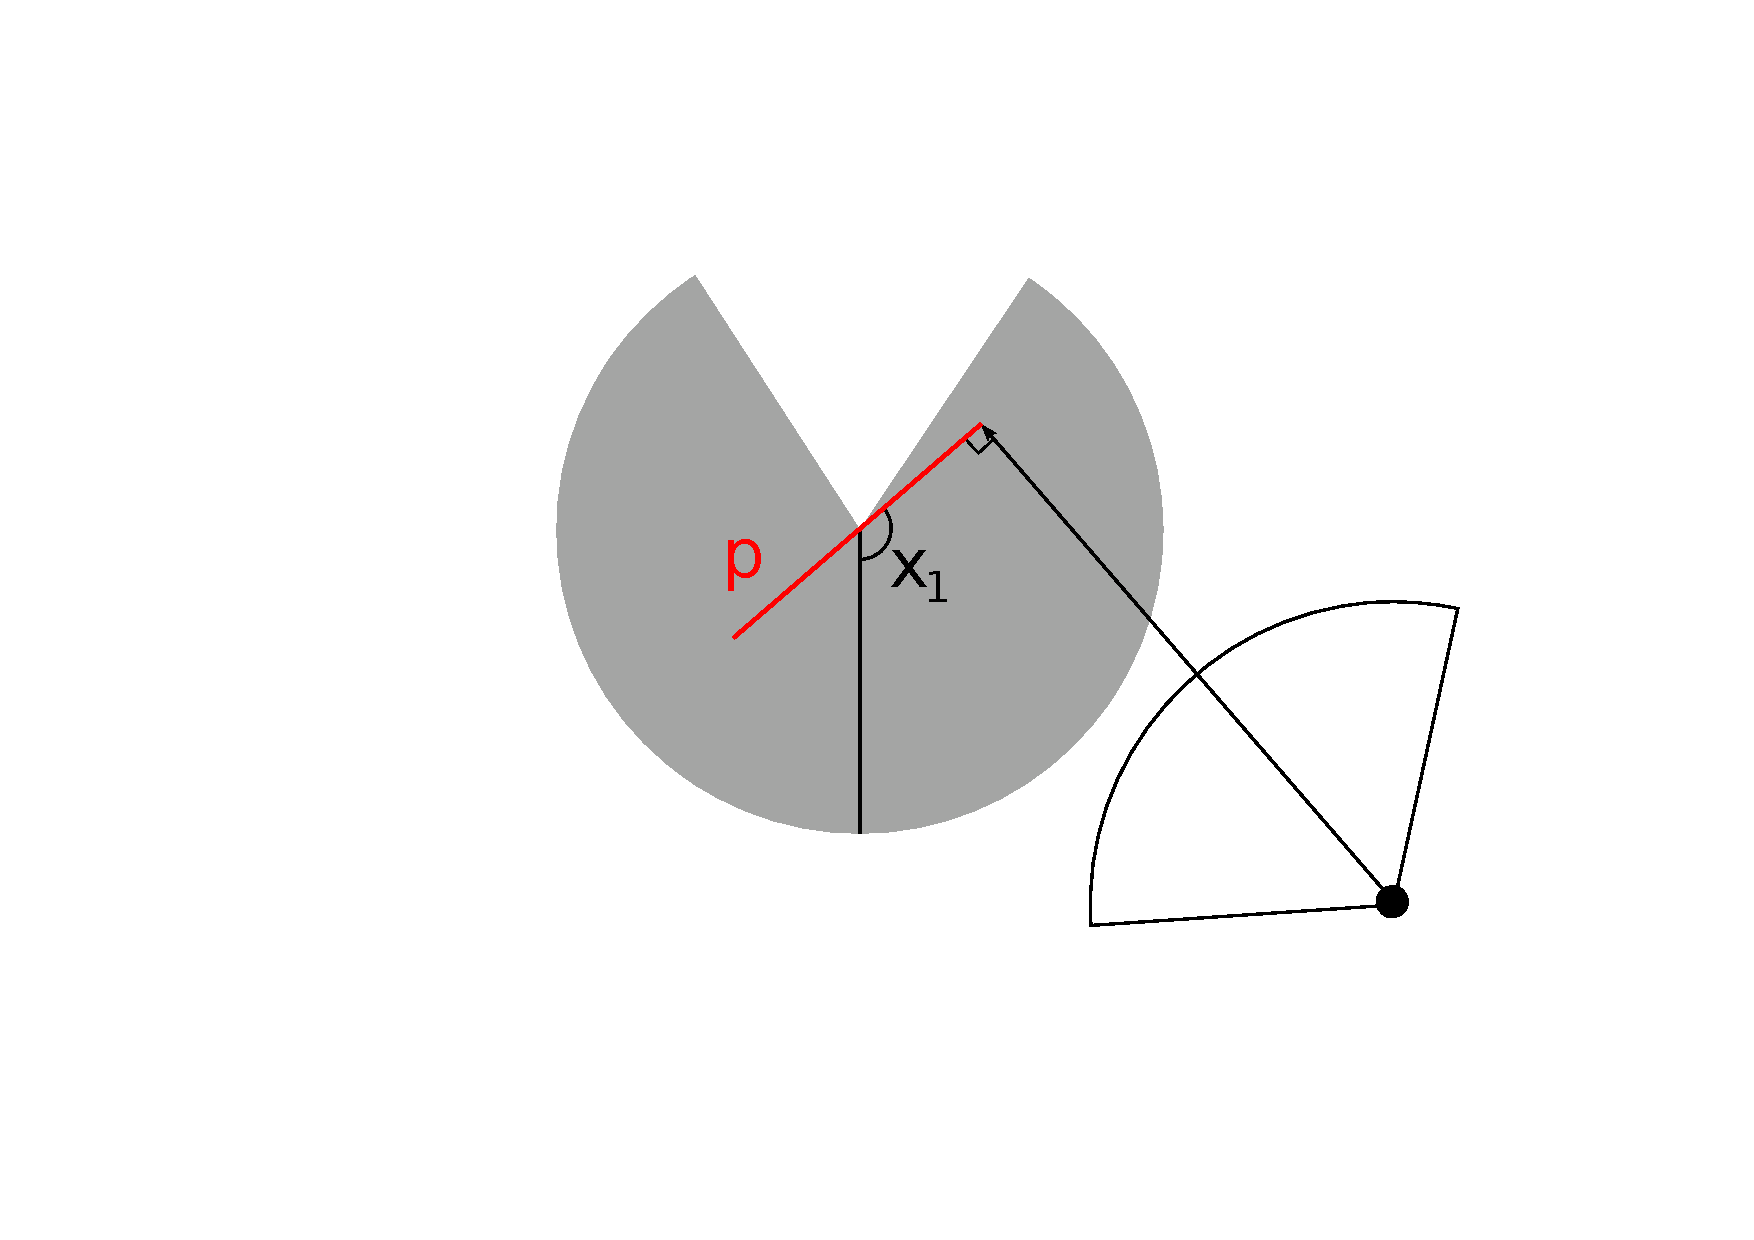
\includegraphics[width=1\textwidth, trim=2cm 1cm 2cm 1cm]{imgs/x1.pdf}
                \caption{$x_1$}               
                \label{f:x1}
        \end{subfigure}
        ~ 
        \begin{subfigure}[t]{0.22\textwidth}
                \centering
        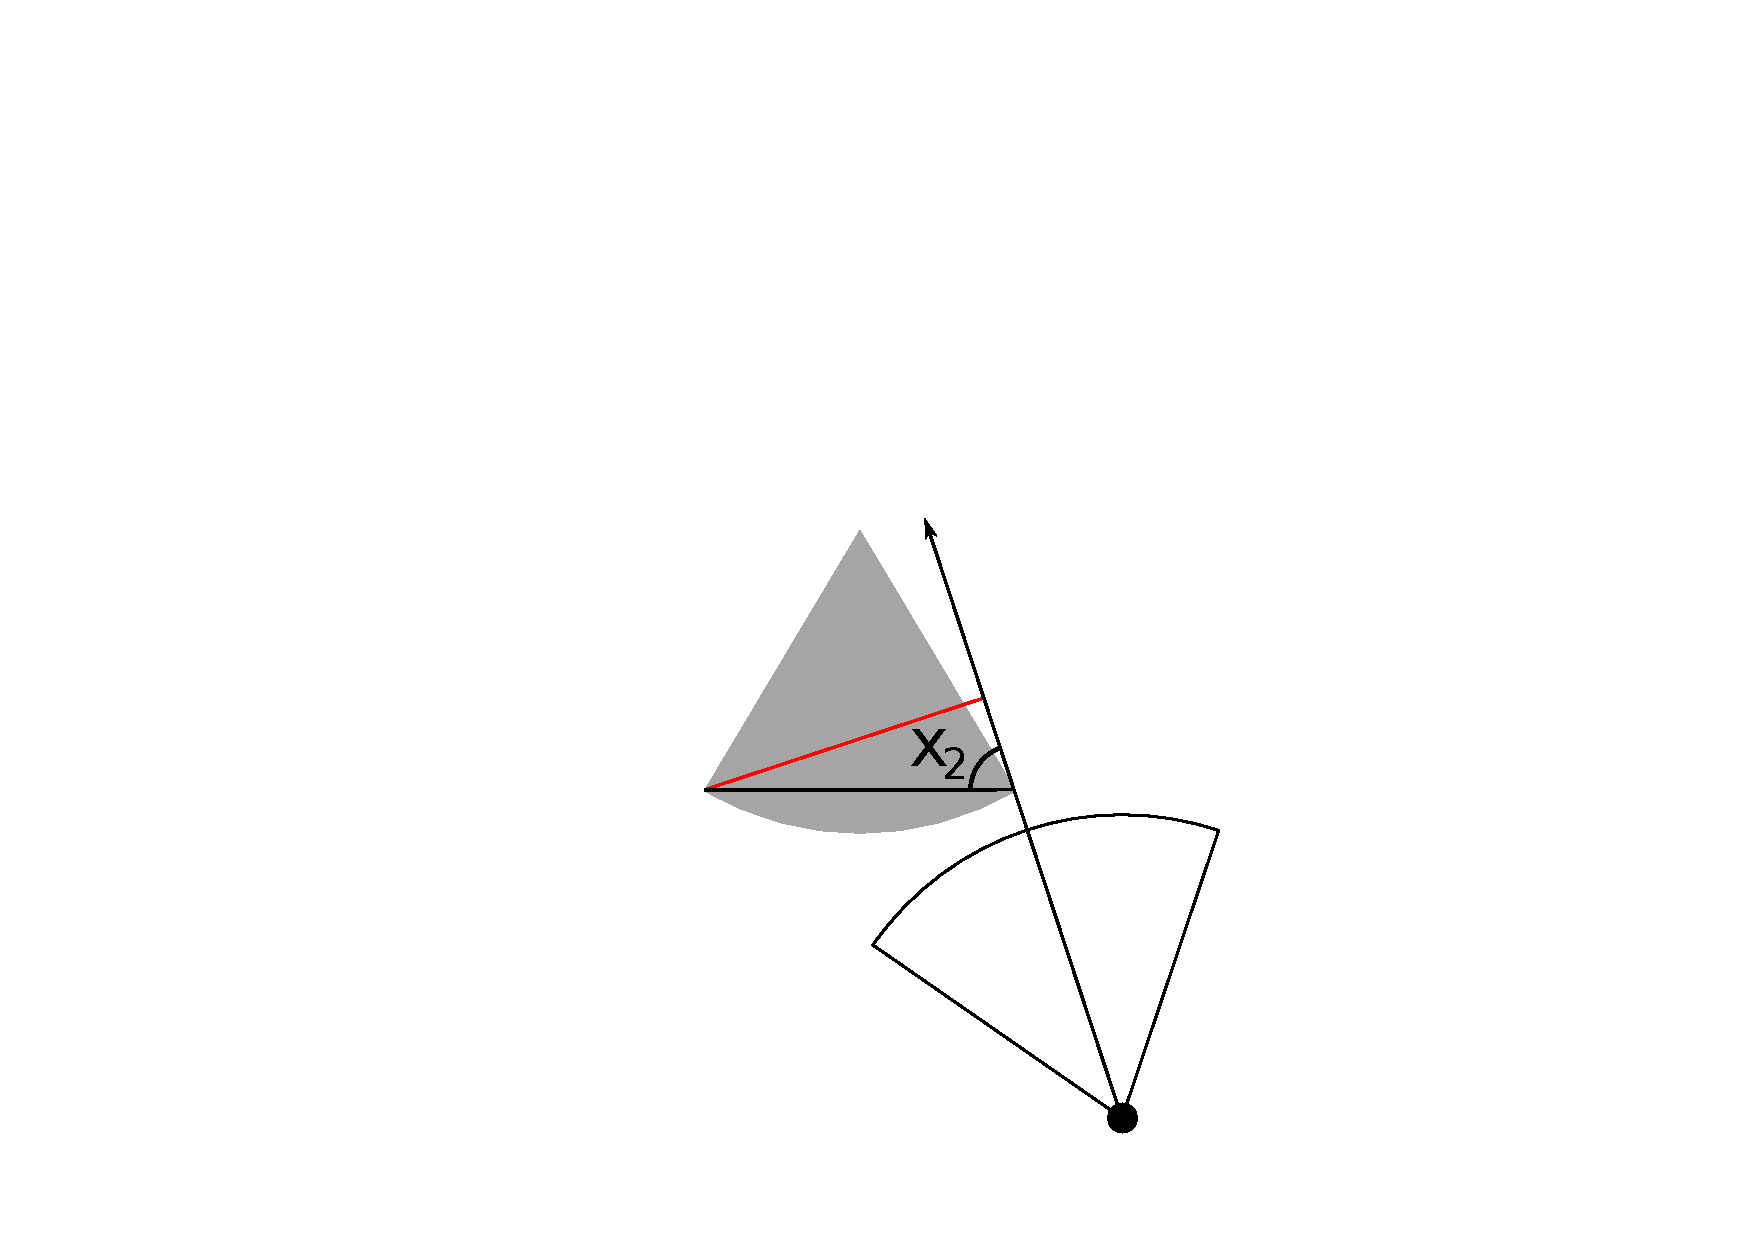
\includegraphics[width=1\textwidth, trim=9cm 2cm 9cm 2cm]{imgs/x2.pdf}
                \caption{$x_2$}               
                \label{f:x2}
        \end{subfigure}
        ~ 
	\begin{subfigure}[t]{0.22\textwidth}
                \centering
        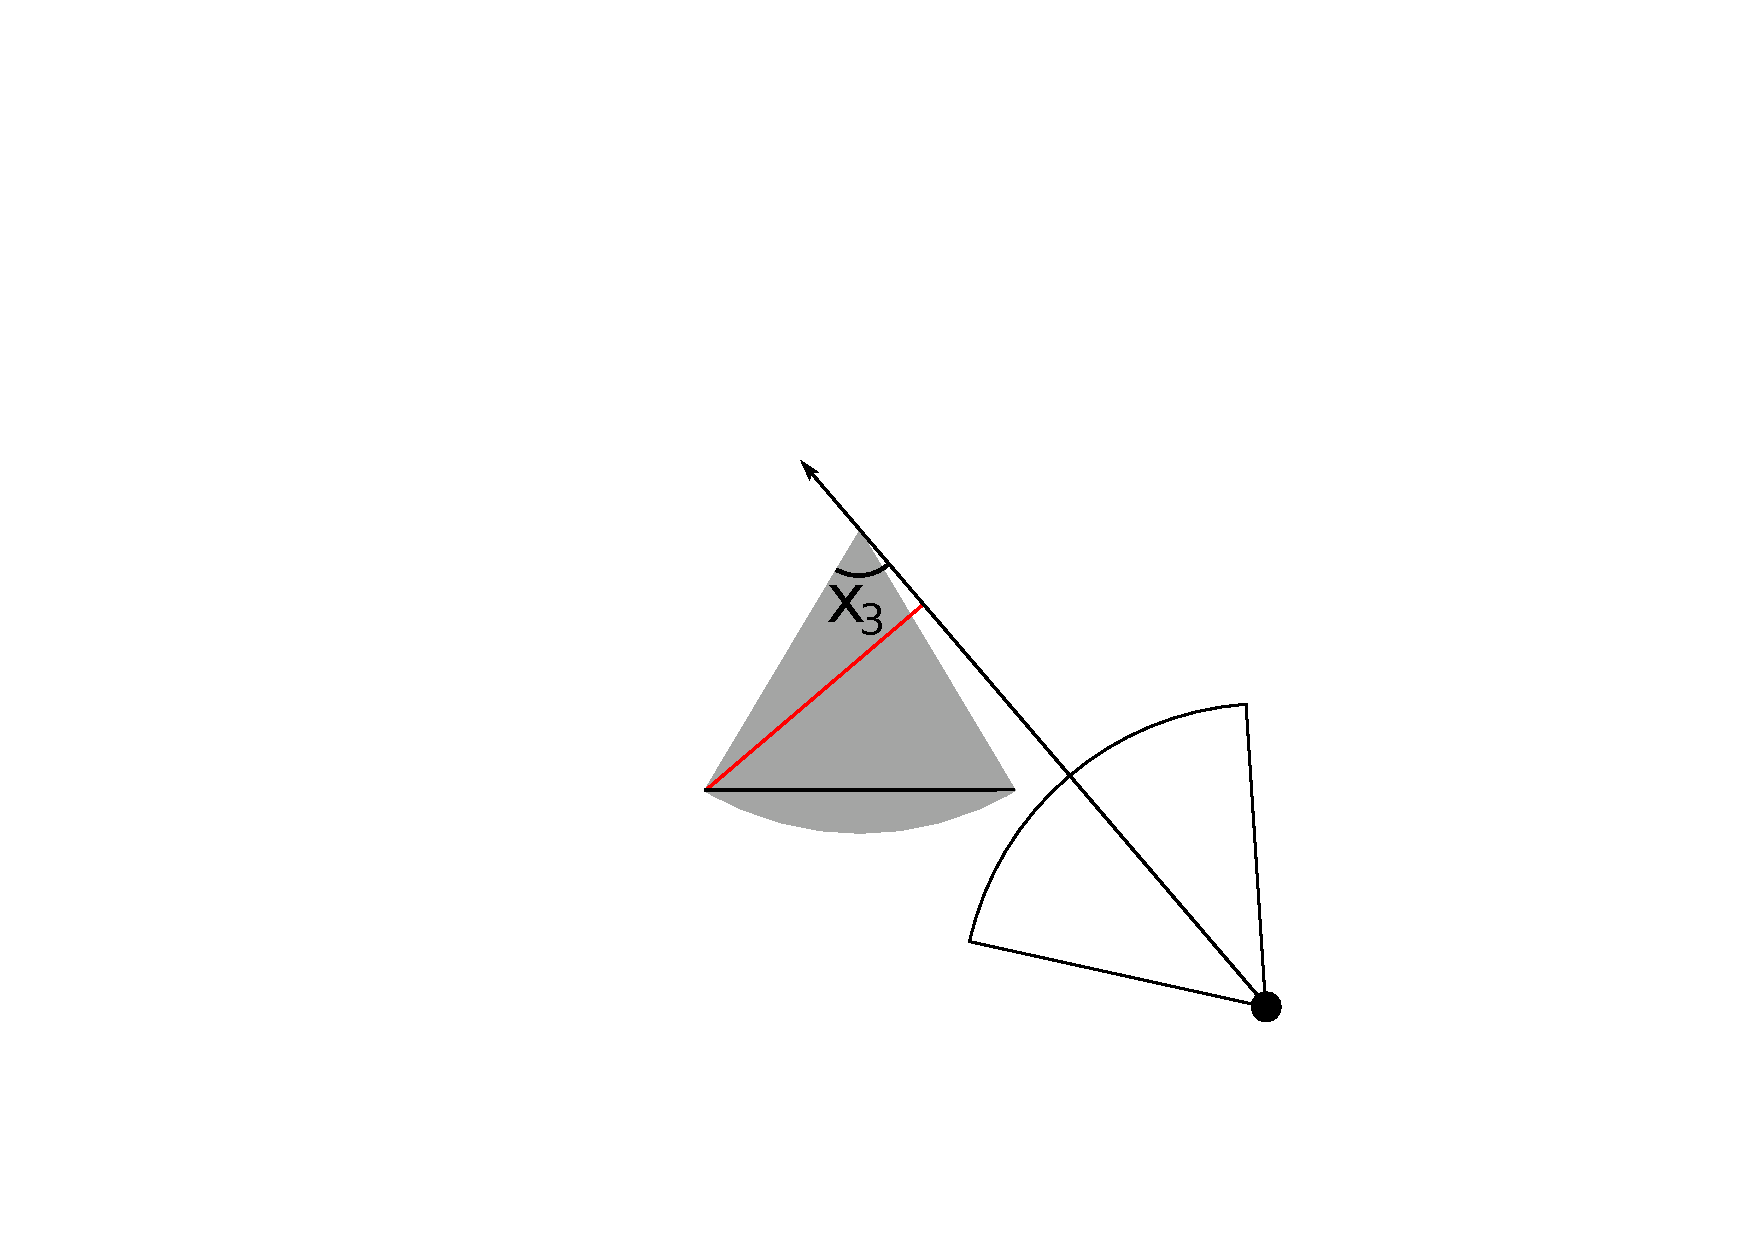
\includegraphics[width=1\textwidth, trim=9cm 2cm 9cm 2cm]{imgs/x3.pdf}
                \caption{$x_3$}               
                \label{f:x3}
        \end{subfigure}%%
	~
	\begin{subfigure}[t]{0.22\textwidth}
                \centering
        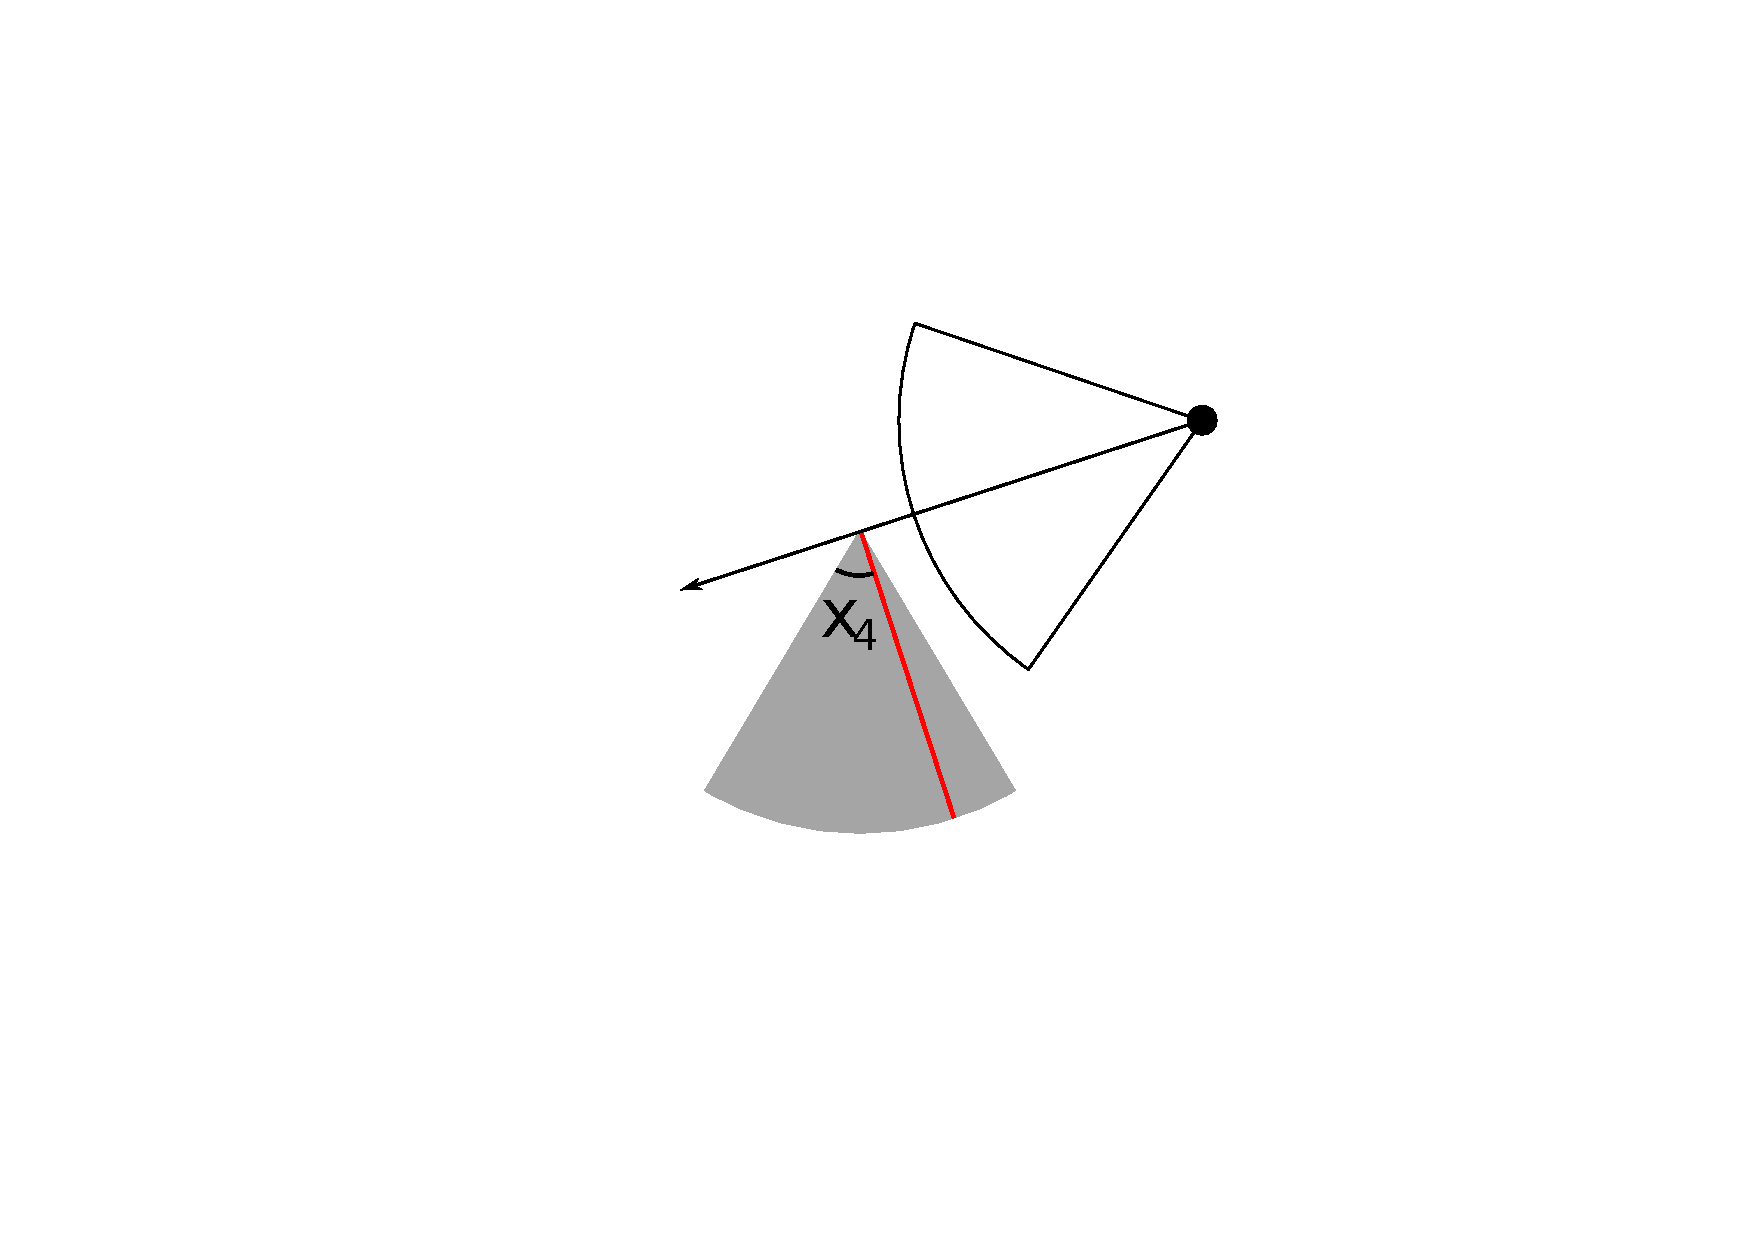
\includegraphics[width=1\textwidth, trim=9cm 2cm 9cm 2cm]{imgs/x4.pdf}
                \caption{$x_4$}               
                \label{f:x4}
        \end{subfigure}%%
\caption{The location of the focal angles $x_{i\in[1,4]}$. In these figures, the sector shaped detection region is shown in grey. Animals are filled black circles and the animal signal is an unfilled sector. The animals direction of movement is indicated with an arrow. The profile $p$ is shown with a red line.}
\label{f:xis}
\end{figure}



There are three submodels within quadrant NE. Note that NE1 covers the area $\alpha=2\pi$ as well as the triangle below it as these two models are specified exactly the same, rather than happening to have equal results.

These models have up to five profiles.

\begin{enumerate}
\item The profile width starts, from $x_1=\frac{\pi}{2}$ as $2r$. 
\item At $x_1 = \theta/2$, the right hand side of the profile cannot be $r$ wide as the corner of the `blind spot' limits its size to being $r\cos(x_1 - \theta/2)$ wide (see Fig.~\ref{f:NELimit}). 

\item The third profile is only found in NE3. If $\alpha < 4\pi - 2\theta$, then at $x_1=\theta/2$, when the profile is perpendicular to the edge of the blind spot, the whole right side of the profile is invisible to the sensor (see Fig.~\ref{f:NE3third}). This gives a profile size of just $r$.

\item At some point, the sensor can detect animals once they have passed the blind spot giving a profile width of $r + r\cos(x_1 + \theta/2)$. From $x_1=\pi$, if the animal call is wide enough to be detected in this area, this is the wider profile. This then defines the split between NE1 and NE2. In NE1, with $\alpha > 3\pi - \theta$, the animal call is wide enough that at $x_1=\pi$ the animal can already be detected past the blind spot and so this profile is used. In NE2, with $\alpha < 3\pi - \theta$, the latter profile is reached at $5\pi/2 - \theta/2 - \alpha/2$ and is therefore dependant on the sizes of $\alpha$ and $\theta$. 

\item Finally, common to all three models, at $x_1 = 2\pi - \theta/2$ the profile becomes a full $2r$ once again. \label{NElist5}
\end{enumerate}



\subsubsection{Model NE1} \label{NE1}

Submodel NE1 exists within the area bounded by $\alpha\le2\pi$, $\theta\le2\pi$ and $\alpha \ge 3\pi - \theta$. It has four profiles; it does not include the $r$ profile at $x_1=\pi$. Furthermore, $\theta$ is wide enough that the $r + r\cos(x_1 + \theta/2)$ profile starts at $\pi$. This then gives us


\begin{align}
    \bar{p}_{\text{\tiny{NE1}}} =&\frac{1}{\pi} \left(\;\;\int\limits_{\frac{\pi}{2}}^{\frac{\theta}{2}}2 r\;\mathrm{d}x_{1}+\int\limits_{\frac{\theta}{2}}^{\pi}r \cos{\left (\frac{\theta}{2} - x_{1} \right )} + r\;\mathrm{d}x_{1}\right.\notag\\
 &\left.+\int\limits_{\pi}^{2 \pi - \frac{\theta}{2}}r \cos{\left (\frac{\theta}{2} + x_{1} \right )} + r\;\mathrm{d}x_{1}+\int\limits_{2 \pi - \frac{\theta}{2}}^{\frac{3 \pi}{2}}2 r\;\mathrm{d}x_{1}\right)\label{pNE1Def}\\
    \bar{p}_{\text{\tiny{NE1}}}  =& \frac{r}{\pi} \left(\theta + 2 \sin{\left (\frac{\theta}{2} \right )}\right)\label{pNE1Sln}
\end{align}





\subsubsection{Model NE2} \label{NE2}

Model NE2 is bounded by $\alpha \le 3\pi - \theta$, $\alpha \ge 4\pi - 2\theta$ and $\alpha \ge \pi$. It is the same as NE1 except that the third profile starts at $5\pi/2 - \theta/2 - \alpha/2$ instead of at $\pi$ which is reflected in the different bounds in the second and third integral.

\begin{align}
    \bar{p}_{\text{\tiny{NE2}}} =&\frac{1}{\pi} \left(\;\;\int\limits_{\frac{\pi}{2}}^{\frac{\theta}{2}}2 r\;\mathrm{d}x_{1}+\int\limits_{\frac{\theta}{2}}^{\frac{5 \pi}{2} - \frac{\theta}{2} - \frac{\alpha}{2}}r \cos{\left (\frac{\theta}{2} - x_{1} \right )} + r\;\mathrm{d}x_{1}\right.\notag\\
 &\left.+\int\limits_{\frac{5 \pi}{2} - \frac{\theta}{2} - \frac{\alpha}{2}}^{2 \pi - \frac{\theta}{2}}r \cos{\left (\frac{\theta}{2} + x_{1} \right )} + r\;\mathrm{d}x_{1}+\int\limits_{2 \pi - \frac{\theta}{2}}^{\frac{3 \pi}{2}}2 r\;\mathrm{d}x_{1}\right)\label{pNE2Def}\\
    \bar{p}_{\text{\tiny{NE2}}}  =& \frac{r}{\pi} \left(\theta - \cos{\left (\frac{\alpha}{2} \right )} + \cos{\left (\frac{\alpha}{2} + \theta \right )}\right)\label{pNE2Sln}
\end{align}

\subsubsection{Model NE3} \label{NE3}

Model NE3 is bound by $\alpha \le 4\pi - 2\theta$, $\alpha \ge \pi$ and $\theta \ge \pi$. It is the same as NE2 except that it contains the extra profile with width $r$ (third integral).

\begin{align}
    \mathrm{pNE3} =&\frac{1}{\pi} \left(\;\;\int\limits_{\frac{\pi}{2}}^{\frac{\theta}{2}}2 r\;\mathrm{d}x_{1}+\int\limits_{\frac{\theta}{2}}^{\frac{\pi}{2} + \frac{\theta}{2}}r + r \cos{\left (- x_{1} + \frac{\theta}{2} \right )}\;\mathrm{d}x_{1}\right.\notag\\
 &\left.+\int\limits_{\frac{\pi}{2} + \frac{\theta}{2}}^{\frac{5 \pi}{2} - \frac{\theta}{2} - \frac{\alpha}{2}}r\;\mathrm{d}x_{1}+\int\limits_{\frac{5 \pi}{2} - \frac{\theta}{2} - \frac{\alpha}{2}}^{2 \pi - \frac{\theta}{2}}r + r \cos{\left (x_{1} + \frac{\theta}{2} \right )}\;\mathrm{d}x_{1}+\int\limits_{2 \pi - \frac{\theta}{2}}^{\frac{3 \pi}{2}}2 r\;\mathrm{d}x_{1}\right)\label{pNE3Def}\\
    \mathrm{pNE3} =& \frac{r}{\pi} \left(\theta - \cos{\left (\frac{\alpha}{2} \right )} + 1\right)\label{pNE3Sln}
\end{align}



\begin{figure}[t]
        \centering
        \begin{subfigure}[t]{0.3\textwidth}
                \centering
        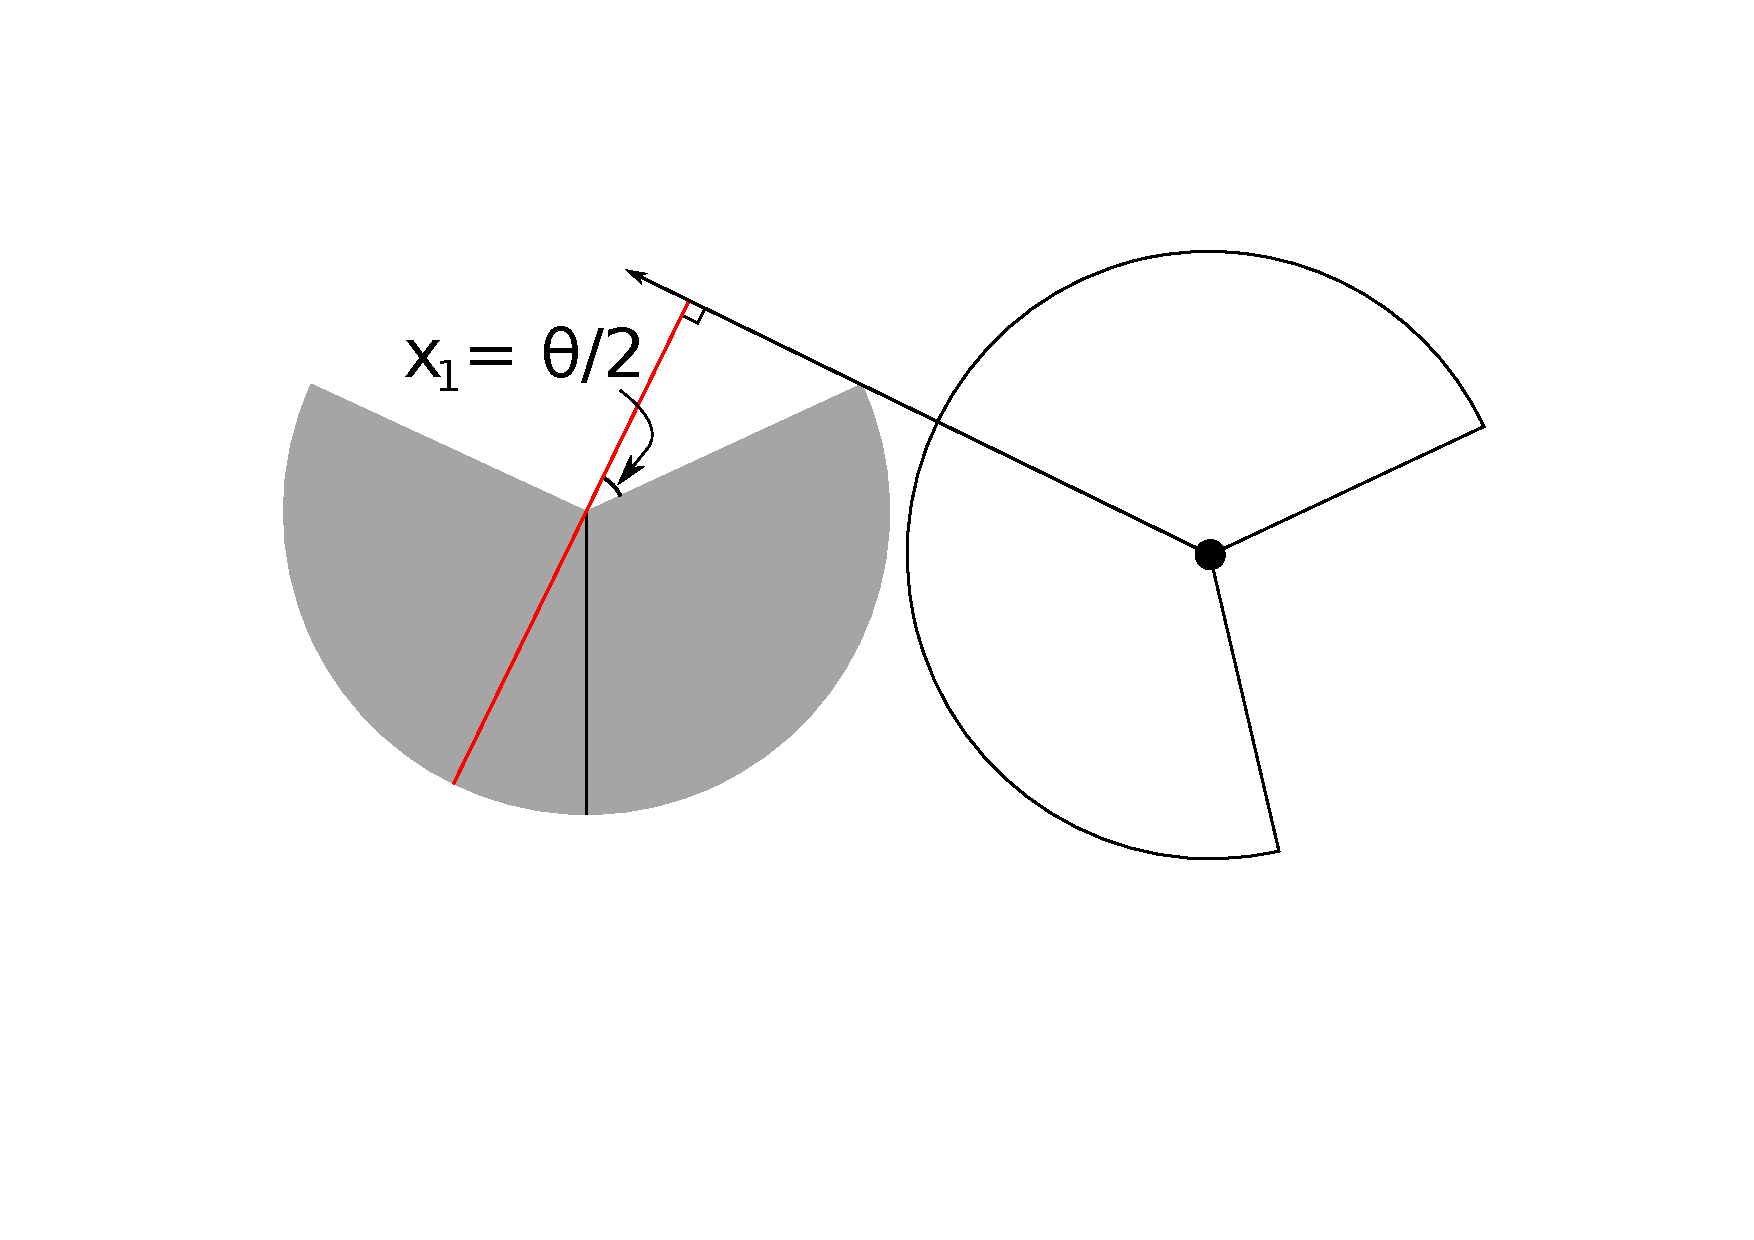
\includegraphics[width=1\textwidth, trim=5cm 3cm 4cm 1cm]{imgs/ne2.pdf}
                \caption{}
                \label{f:NELimit}
        \end{subfigure}
        ~ 
        \begin{subfigure}[t]{0.3\textwidth}
                \centering
                       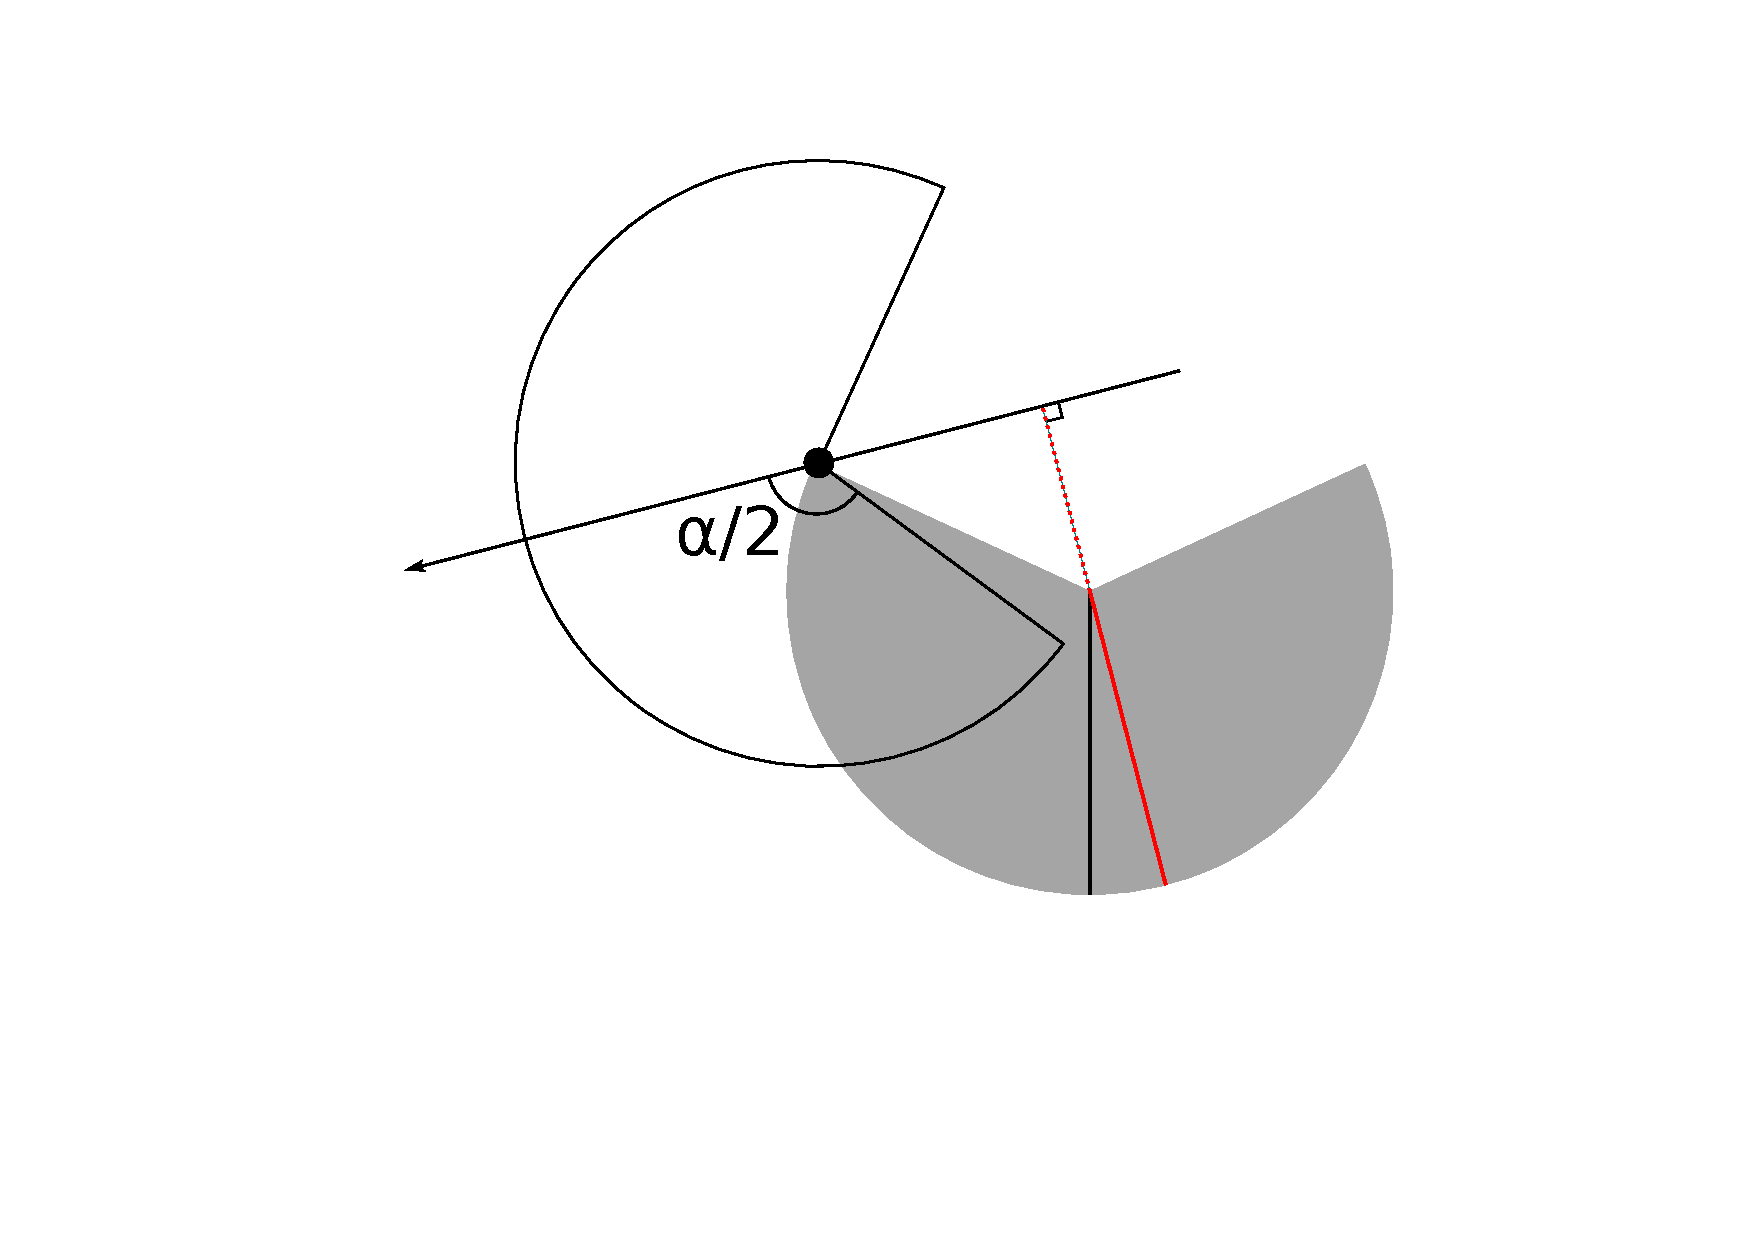
\includegraphics[width=1\textwidth, trim=4cm 2cm 6cm 0cm]{imgs/ne33.pdf}
                \caption{}
                \label{f:NE3third}
        \end{subfigure}
        ~ 
        \begin{subfigure}[t]{0.3\textwidth}
                \centering
                       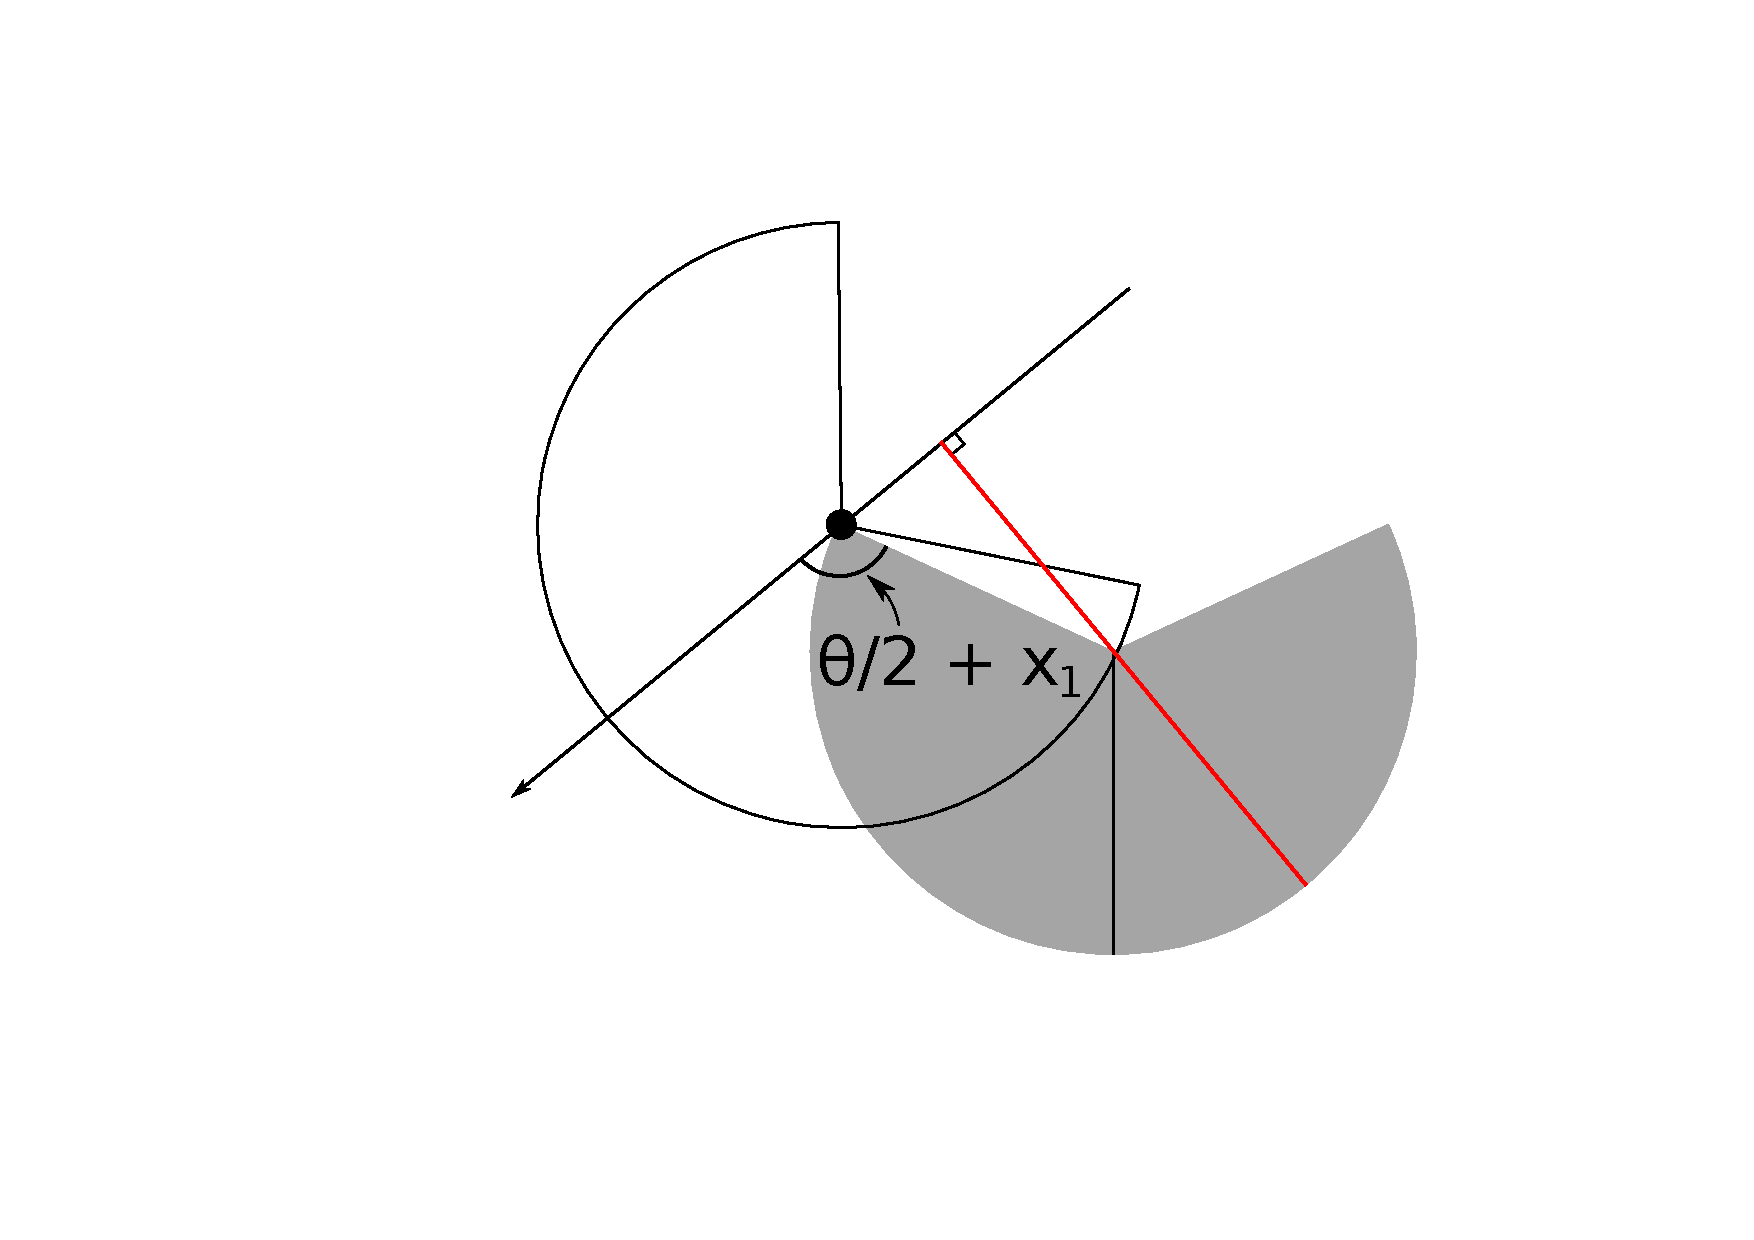
\includegraphics[width=1\textwidth, trim=5cm 1cm 4cm 1cm]{imgs/ne34.pdf}
                \caption{}
                \label{f:NE3fourth}
        \end{subfigure}

\caption{A) The second integral in NE with width $r + r\cos(x_1 - \theta/2)$ B) The third integral in NE3. $\alpha/2$ is labelled. As it is small, animals to the right of the detector cannot be detected (shown by a dashed red line.) C) After further rotation, $\alpha/2$ is now bigger than the angle shown and animals to the right of the detector can again be sensed.   }
\label{f:NE}
\end{figure}


\subsection{Models SE2--4} \label{SE}

Quadrant SE contains three submodels (excluding SE1) that differ in ways reminiscent of the models in NE. There are four possible profiles.
\begin{enumerate}
\item As $\alpha$ is less than $\pi$ the profile is smaller than $2r$, even when the sensor width is a full diameter. The profile width starts as $2r\sin(\alpha/2)$.
\item Similar to NE, at a certain point the blind spot of the sensor area limits the profile width on one side. This gives a profile width of $r\sin(\alpha/2) + r\cos(x_1 - \theta/2)$ (see Fig.~\ref{f:se3}).
\item Also similar to NE, there can be a point where the right side of the profile is 0 giving a profile width of $r\sin(\alpha/2)$. 
\item If $\alpha \le 2\pi - \theta$, then at $x_1 = \theta/2 + \pi/2 + \alpha/2 $ the profile width becomes 0. This inequality distinguishes between SE3 and SE4. 
\item The third profile $r\sin(\alpha/2)$ starts at $\theta/2 + \pi/2$ while at $5\pi/2 - \alpha/2 - \theta/2$ the profile returns to size $2r\sin(\alpha/2)$. If $\theta/2 + \pi/2 \ge 5\pi/2 - \alpha/2 - \theta/2$ we go straight into the  $2r\sin(\alpha/2)$ profile and miss the $r\sin(\alpha/2)$ profile.  SE2 and SE3 are seperated by this inequality which simplifies to $\alpha \le 4\pi - 2\theta$. 

\end{enumerate}



\begin{figure}[t]
        \centering
        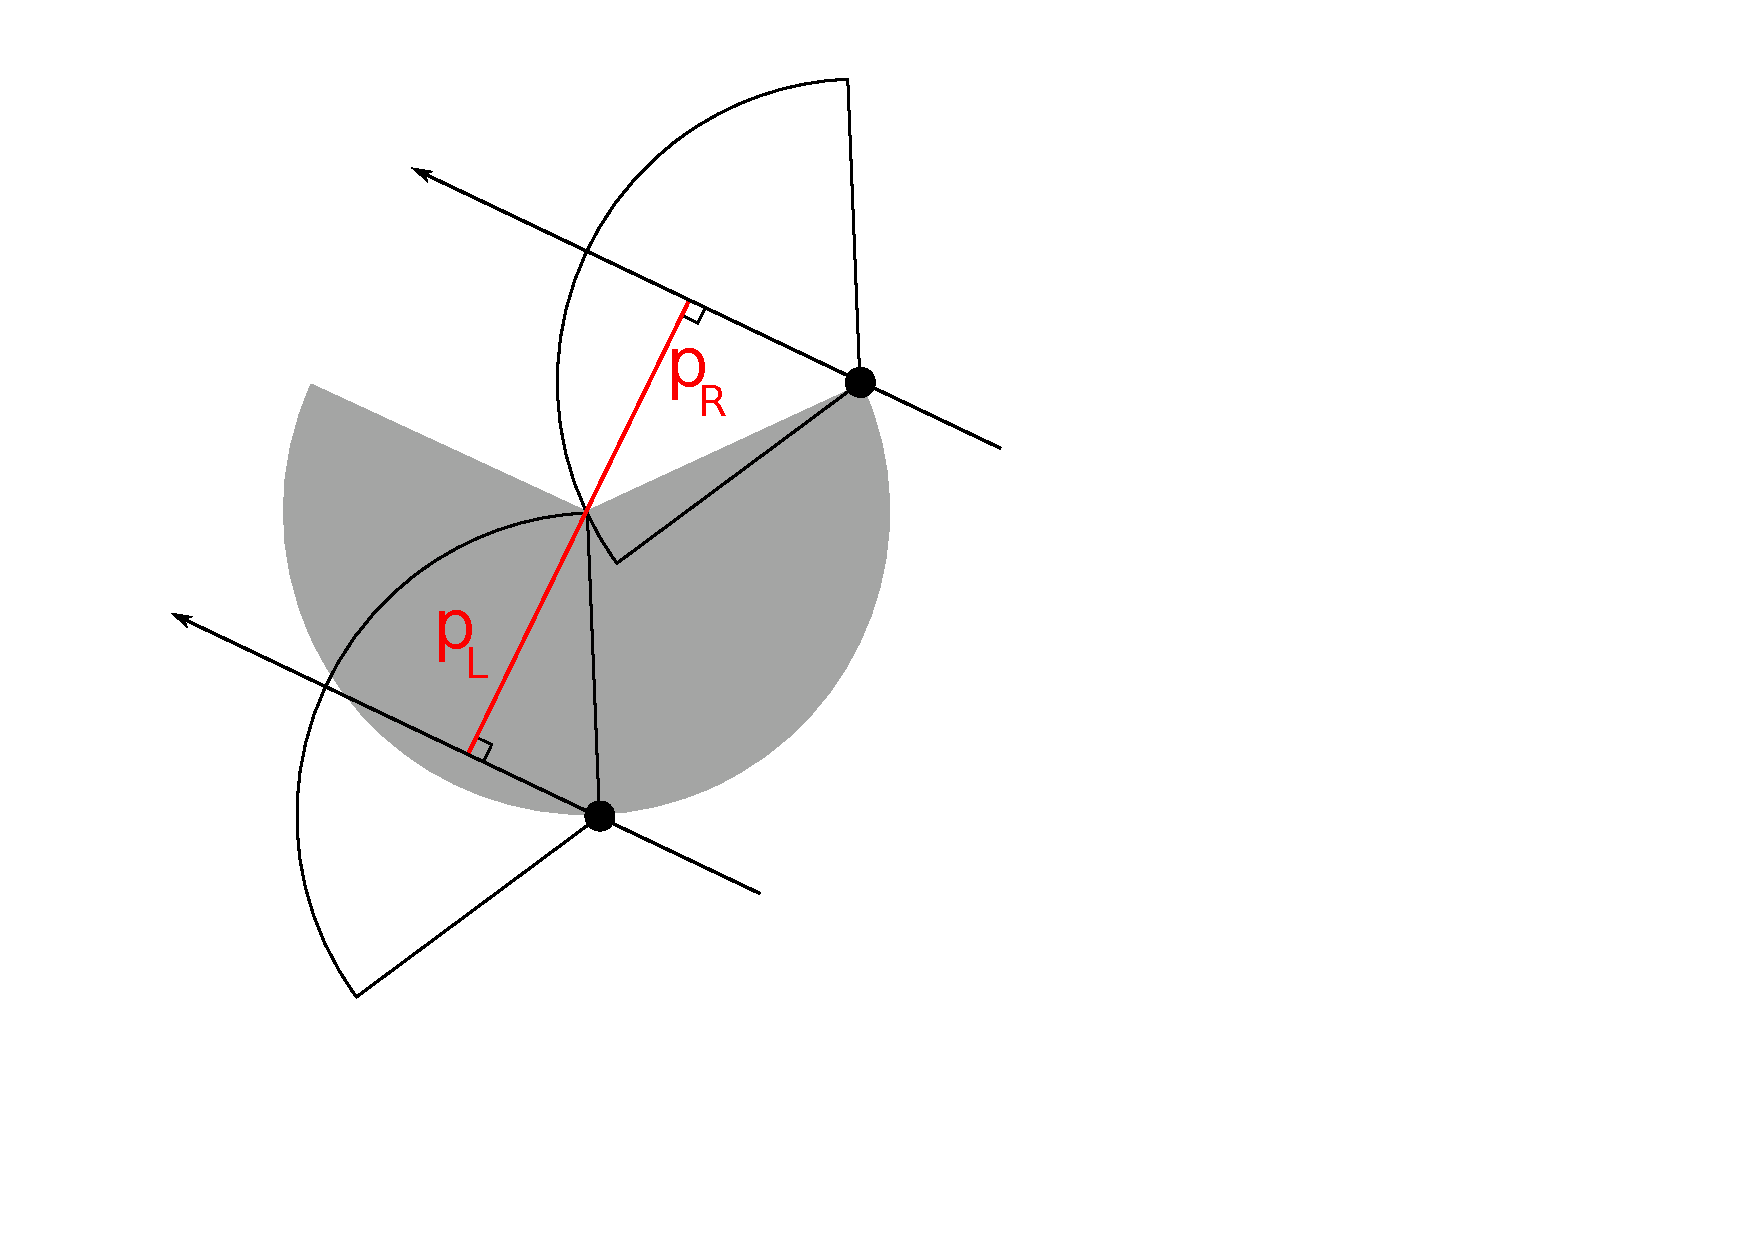
\includegraphics[width=0.35\textwidth, trim=1cm 4cm 9cm 1cm]{imgs/se3.pdf}
\caption{A) The second integral in SE. The right side of the profile ($p_R$) is limited by the size of the sensor region  while the left side of the profile ($p_L$) is limited by the size of the call angle. The full profile has width $p = r\sin(\alpha/2) +r\cos(\theta/2-x_1)$.      }
\label{f:se3}
\end{figure}



\subsubsection{Model SE2} \label{SE2}

SE2 is bounded by $\alpha \ge 4\pi - 2\theta$, $\alpha \le \pi$ and $\theta \le 2\pi$. As $\alpha \ge 4\pi - 2\theta$, there is no $r\sin(\alpha/2)$ profile. As $\alpha \le 4\pi - 2\theta$, the profile returns to $2r\sin(\alpha/2)$ rather than going to 0. These integrals relate to profiles (1), (2) and (5) above.

\begin{align}
    \bar{p}_{\text{\tiny{SE2}}} =&\frac{1}{\pi} \left(\;\;\int\limits_{\frac{\pi}{2}}^{\frac{\pi}{2} + \frac{\theta}{2} - \frac{\alpha}{2}}2 r \sin{\left (\frac{\alpha}{2} \right )}\;\mathrm{d}x_{1}+\int\limits_{\frac{\pi}{2} + \frac{\theta}{2} - \frac{\alpha}{2}}^{\frac{5 \pi}{2} - \frac{\theta}{2} - \frac{\alpha}{2}}r \sin{\left (\frac{\alpha}{2} \right )} + r \cos{\left (\frac{\theta}{2} - x_{1} \right )}\;\mathrm{d}x_{1}+\int\limits_{\frac{5 \pi}{2} - \frac{\theta}{2} - \frac{\alpha}{2}}^{\frac{3 \pi}{2}}2 r \sin{\left (\frac{\alpha}{2} \right )}\;\mathrm{d}x_{1}\right)\label{pSE2Def}\\
    \bar{p}_{\text{\tiny{SE2}}}  =& \frac{r}{\pi} \left(\theta \sin{\left (\frac{\alpha}{2} \right )} - \cos{\left (\frac{\alpha}{2} \right )} + \cos{\left (\frac{\alpha}{2} + \theta \right )}\right)\label{pSE2Sln}
\end{align}


\subsubsection{Model SE3} \label{SE3}

SE3 is bounded by $4\pi - 2\theta \le \alpha \le 4\pi - 2\theta$ and $\alpha \le \pi$. Therefore there is a $r\sin(\alpha/2)$ profile but no $0r$ profile. This relates to profiles (1), (2), (3) and (5) above.

\begin{align}
    \bar{p}_{\text{\tiny{SE3}}} =&\frac{1}{\pi} \left(\;\;\int\limits_{\frac{\pi}{2}}^{\frac{\pi}{2} + \frac{\theta}{2} - \frac{\alpha}{2}}2 r \sin{\left (\frac{\alpha}{2} \right )}\;\mathrm{d}x_{1}+\int\limits_{\frac{\pi}{2} + \frac{\theta}{2} - \frac{\alpha}{2}}^{\frac{\theta}{2} + \frac{\pi}{2}}r \sin{\left (\frac{\alpha}{2} \right )} + r \cos{\left (\frac{\theta}{2} - x_{1} \right )}\;\mathrm{d}x_{1}\right.\notag\\
 &\left.+\int\limits_{\frac{\theta}{2} + \frac{\pi}{2}}^{\frac{5 \pi}{2} - \frac{\theta}{2} - \frac{\alpha}{2}}r \sin{\left (\frac{\alpha}{2} \right )}\;\mathrm{d}x_{1}+\int\limits_{\frac{5 \pi}{2} - \frac{\theta}{2} - \frac{\alpha}{2}}^{\frac{3 \pi}{2}}2 r \sin{\left (\frac{\alpha}{2} \right )}\;\mathrm{d}x_{1}\right)\label{pSE3Def}\\
    \bar{p}_{\text{\tiny{SE3}}}  =& \frac{r}{\pi} \left(\theta \sin{\left (\frac{\alpha}{2} \right )} - \cos{\left (\frac{\alpha}{2} \right )} + 1\right)\label{pSE3Sln}
\end{align}

\subsubsection{Model SE4} \label{SE4}

Finally SE4 is bounded by  $\alpha \le 4\pi - 2\theta $, $\alpha\le\pi$ and $\theta \le \pi$. It is the same as SE3 except that the profile becomes 0 rather than returning to $2r\sin(\alpha/2)$. This relates to profiles (1), (2), (3) and (4) above though profile (4) with width 0 is not shown.

\begin{align}
    \mathrm{pSE4} =&\frac{1}{\pi} \left(\;\;\int\limits_{\frac{\pi}{2}}^{\frac{\pi}{2} + \frac{\theta}{2} - \frac{\alpha}{2}}2 r \sin{\left (\frac{\alpha}{2} \right )}\;\mathrm{d}x_{1}+\int\limits_{\frac{\pi}{2} + \frac{\theta}{2} - \frac{\alpha}{2}}^{\frac{\pi}{2} + \frac{\theta}{2}}r \cos{\left (- x_{1} + \frac{\theta}{2} \right )} + r \sin{\left (\frac{\alpha}{2} \right )}\;\mathrm{d}x_{1}+\int\limits_{\frac{\pi}{2} + \frac{\theta}{2}}^{\frac{\pi}{2} + \frac{\theta}{2} + \frac{\alpha}{2}}r \sin{\left (\frac{\alpha}{2} \right )}\;\mathrm{d}x_{1}\right)\label{pSE4Def}\\
    \mathrm{pSE4} =& \frac{r}{\pi} \left(\theta \sin{\left (\frac{\alpha}{2} \right )} - \cos{\left (\frac{\alpha}{2} \right )} + 1\right)\label{pSE4Sln}
\end{align}


\begin{figure}[t]
        \centering
        \begin{subfigure}[t]{0.35\textwidth}
                \centering
        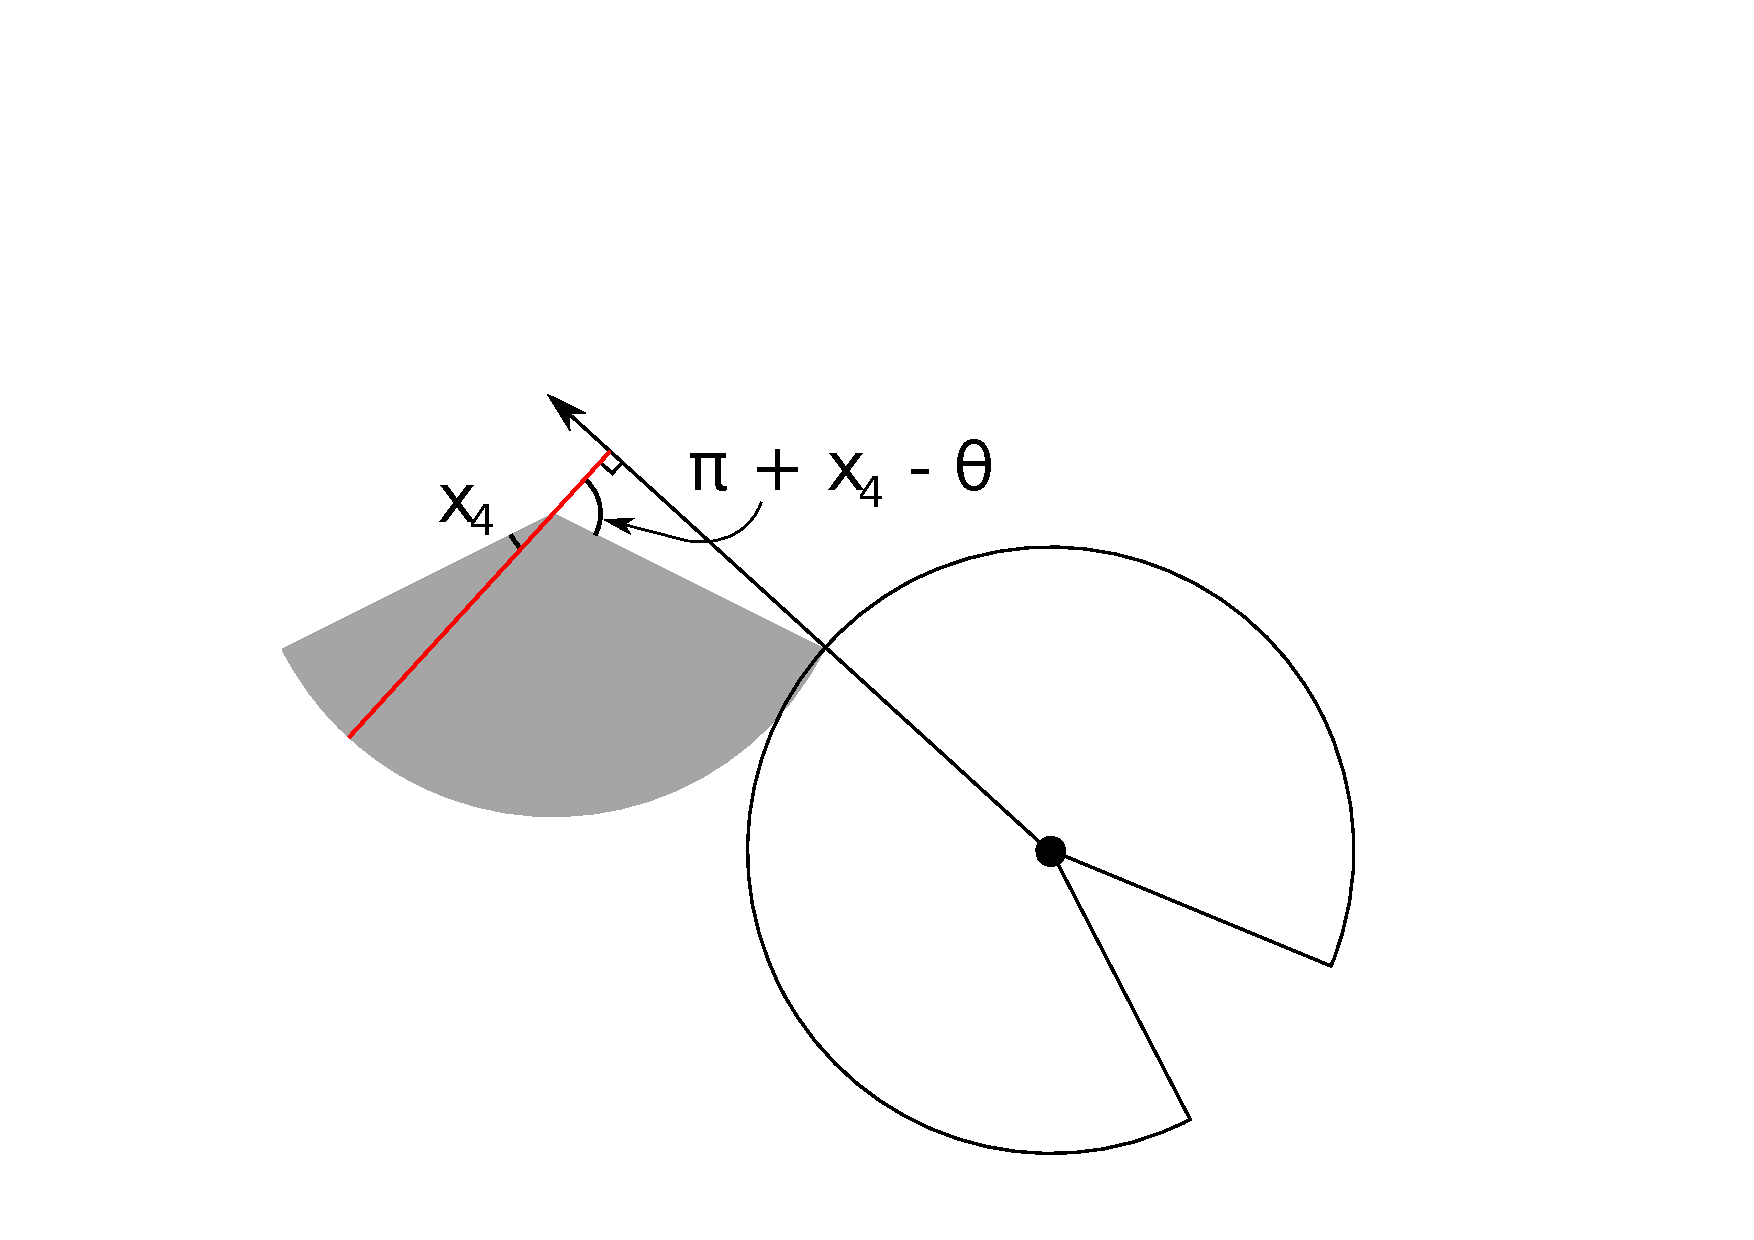
\includegraphics[width=1\textwidth, trim=5cm 1cm 4cm 1cm]{imgs/nw2.pdf}
                \caption{}
                \label{f:NW1AT}
        \end{subfigure}
~ 
        \begin{subfigure}[t]{0.35\textwidth}
                \centering
        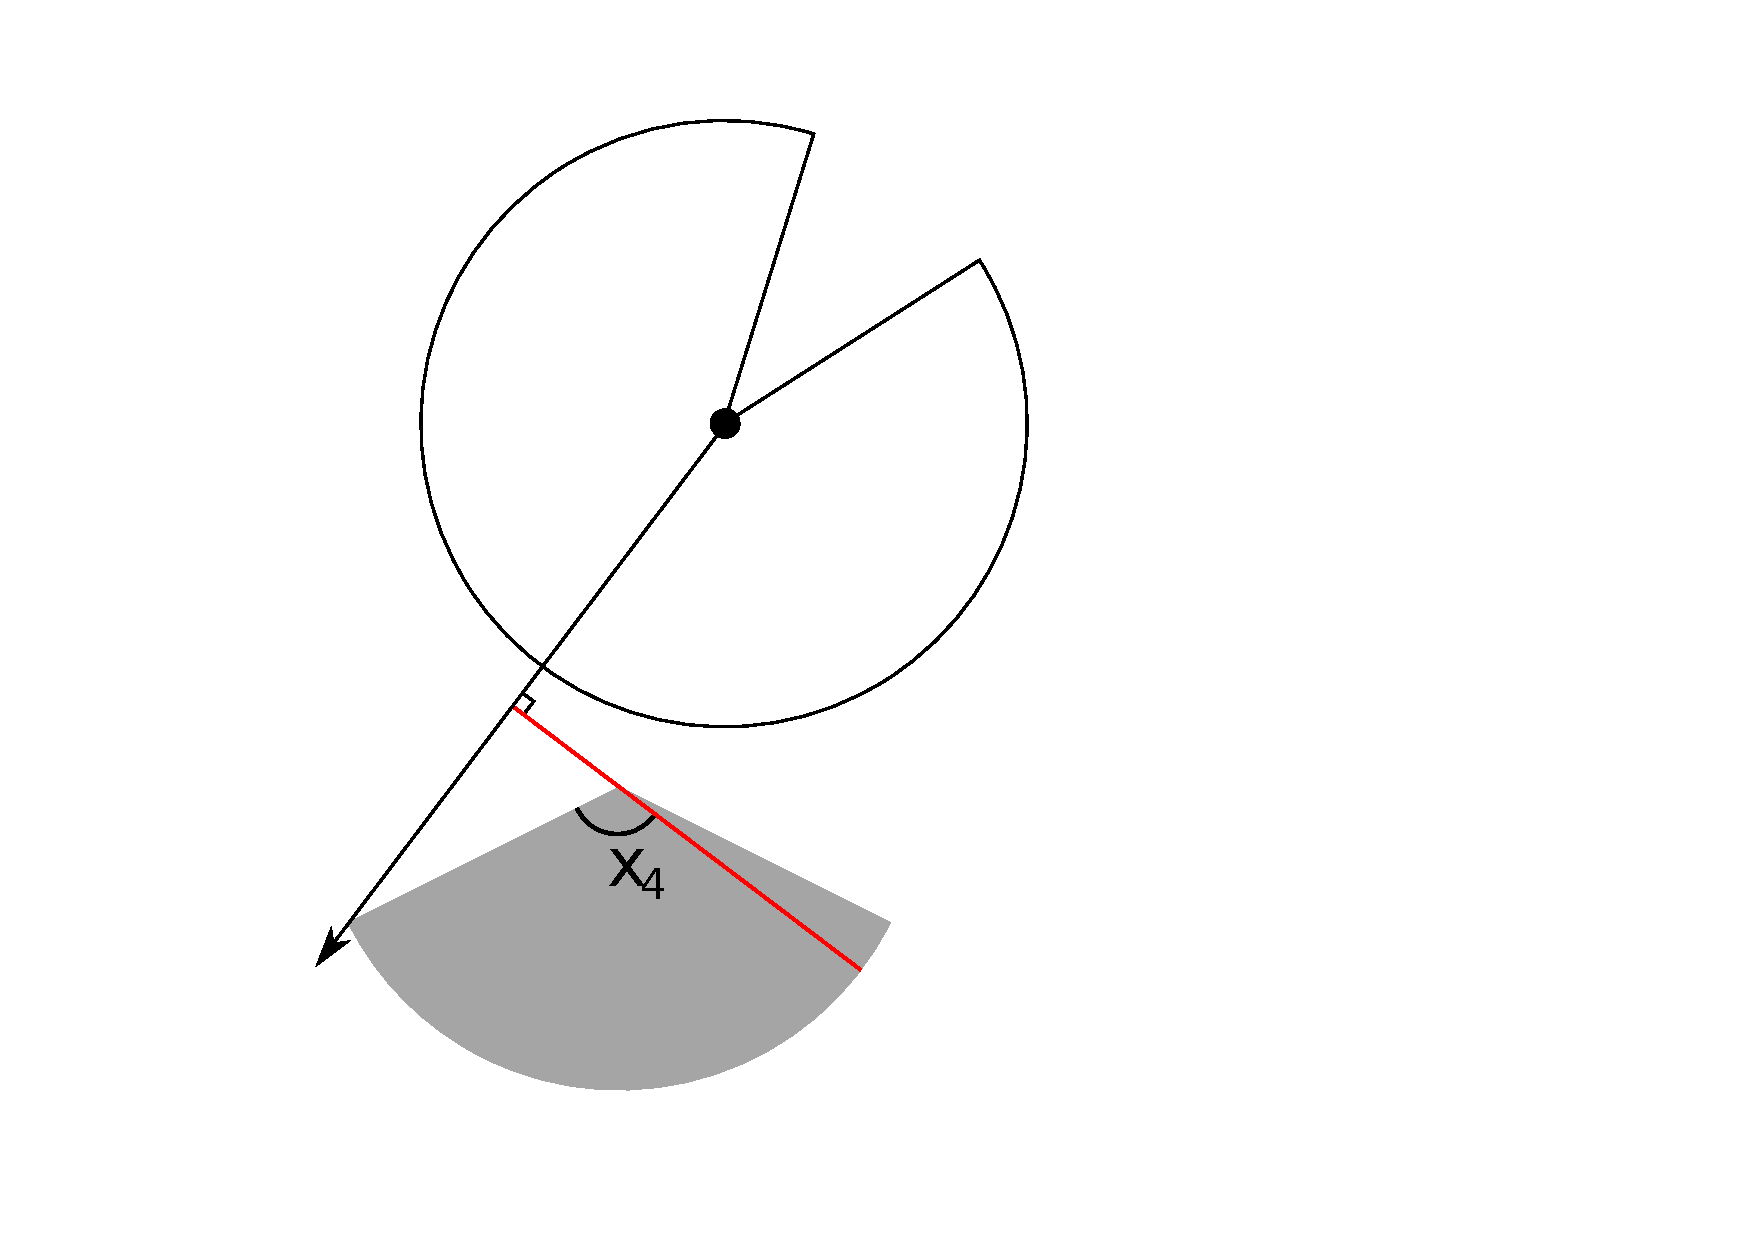
\includegraphics[width=1\textwidth, trim=0cm 1cm 4cm 1cm]{imgs/nw4.pdf}
                \caption{}
                \label{f:NW1behindFull}
        \end{subfigure}
\caption{A) and B) The second and fourth profiles of NW1. The left side of of both profiles is of width $r$ while the right side is $r\cos(\pi+x_4-\theta) = - r\cos(\theta - x_4 )$ and $r\cos(\pi-x_4) = - r\cos x_4$ respectively. }
\label{f:NW1}
\end{figure}

\subsection{Model NW1} \label{NW1}

NW1 is the first model with $\theta < \pi$. Whereas previously the focal angle has always been $x_1$, we now use different focal angles. $x_2$ and $x_3$ correspond to $\gamma_1$ and $\gamma_2$ in \cite{rowcliffe2008estimating} while $x_4$ is new. They are described in Fig.~\ref{f:xis}. 

There are five different profiles in NW1.
\begin{enumerate}
\item $x_2$ has an interval of $[\pi/2, \theta/2]$ which is from the angle of approach being directly towards the sensor until the profile is parellel to the left hand radius of the sensor sector. During this interval the profile width is $2r\sin\left(\theta/2\right)\sin(x_2)$ which is calculated using the equation for the length of a chord (see Fig.~\ref{f:x2}). Note that while rotating anti-clockwise (as usual) $x_2$ decreases in size.
\item From here, we examine focal angle $x_4$ (note that $x_3$ is used in later models, but is not relevant here.)  The left side of the profile is a full radius while the right side is limited to $- r\cos(x_4 - \theta)$ (see Fig.~\ref{f:NW1AT}).
\item At $x_4 =  \theta - \pi/2$, the profile is perpendicular to the edge of the sensor area. Here, the right side of the profile is $0r$ giving a profile size of $r$.   %@tim is left side r?
\item When $x_4 = \pi/2$ the angle of approach is from behind the sensor, but we can once again be detected on the right side of the sensor (see Fig.~\ref{f:NW1behindFull}). Therefore the width of the profile is $r - r\cos(x_4)$.
\item  Finally, we have the $x_2$ profile, but from behind. 
\end{enumerate}



\begin{align}
    \mathrm{pNW1} =&\frac{1}{\pi} \left(\;\;\int\limits_{\frac{\theta}{2}}^{\frac{\pi}{2}}2 r \sin{\left (\frac{\theta}{2} \right )} \sin{\left (x_{2} \right )}\;\mathrm{d}x_{2}+\int\limits_{0}^{- \frac{\pi}{2} + \theta}r - r \cos{\left (- x_{4} + \theta \right )}\;\mathrm{d}x_{4}\right.\notag\\
 &\left.+\int\limits_{- \frac{\pi}{2} + \theta}^{\frac{\pi}{2}}r\;\mathrm{d}x_{4}+\int\limits_{\frac{\pi}{2}}^{\theta}r - r \cos{\left (x_{4} \right )}\;\mathrm{d}x_{4}+\int\limits_{\frac{\theta}{2}}^{\frac{\pi}{2}}2 r \sin{\left (\frac{\theta}{2} \right )} \sin{\left (x_{2} \right )}\;\mathrm{d}x_{2}\right)\label{pNW1Def}\\
    \mathrm{pNW1} =& \frac{r}{\pi} \left(\theta + 2\right)\label{pNW1Sln}
\end{align}

\subsection{Models NW2--4} \label{NW2--4}
% @tim this is still crap
The models NW2--4 have the five potential profiles in NW1 but not all profiles occur in each model, and the angle at which transitions occur are different. Furthermore, there is one extra profile possible. 
\begin{enumerate}
\item When approaching the sensor from behind, there is a period where the profile is $r$ wide as in NW1 profile (3). 
\item At some point the right side of the profile becomes viable again. If this occurs in the $x_4$ region, the profile width becomes  $r - r\cos(x_4)$ as in NW1.
\item However, as $\alpha$ is now less than $2\pi$, the right side of the profile might not be viable until we are in the second $x_2$ region. In this case, when we first enter the second $x_2$ region, the profile has a width of $r\cos(x_2 - \theta/2)$. This occurs only if $\alpha \le 3\pi - 2\theta$. This is inequality is found by noting that the right side of the profile become viable at $x_4 = 3\pi/2 - \alpha$ but the $x_2$ region starts at $x_4 = \theta$. The new profile in $x_2$ will only occur if  $ \theta < 3\pi/2 - \alpha/2$ which is rearranged to find the inequality above. This defines the boundary between NW2 and NW3.
\item As $\alpha \le 2\pi$ it is possible that when the angle of approach is from directly behind the sensor the animal will not be detected at all. This is the case if $\alpha/2\le \pi-\theta/2$ as shown in Fig.~\ref{f:NW2--4}. This inequality (simplified as $\alpha\le 2\pi-\theta$) defines the boundary between NW3 and NW4.
\end{enumerate}



\begin{figure}[t]
        \centering
        \begin{subfigure}[t]{0.35\textwidth}
                \centering
        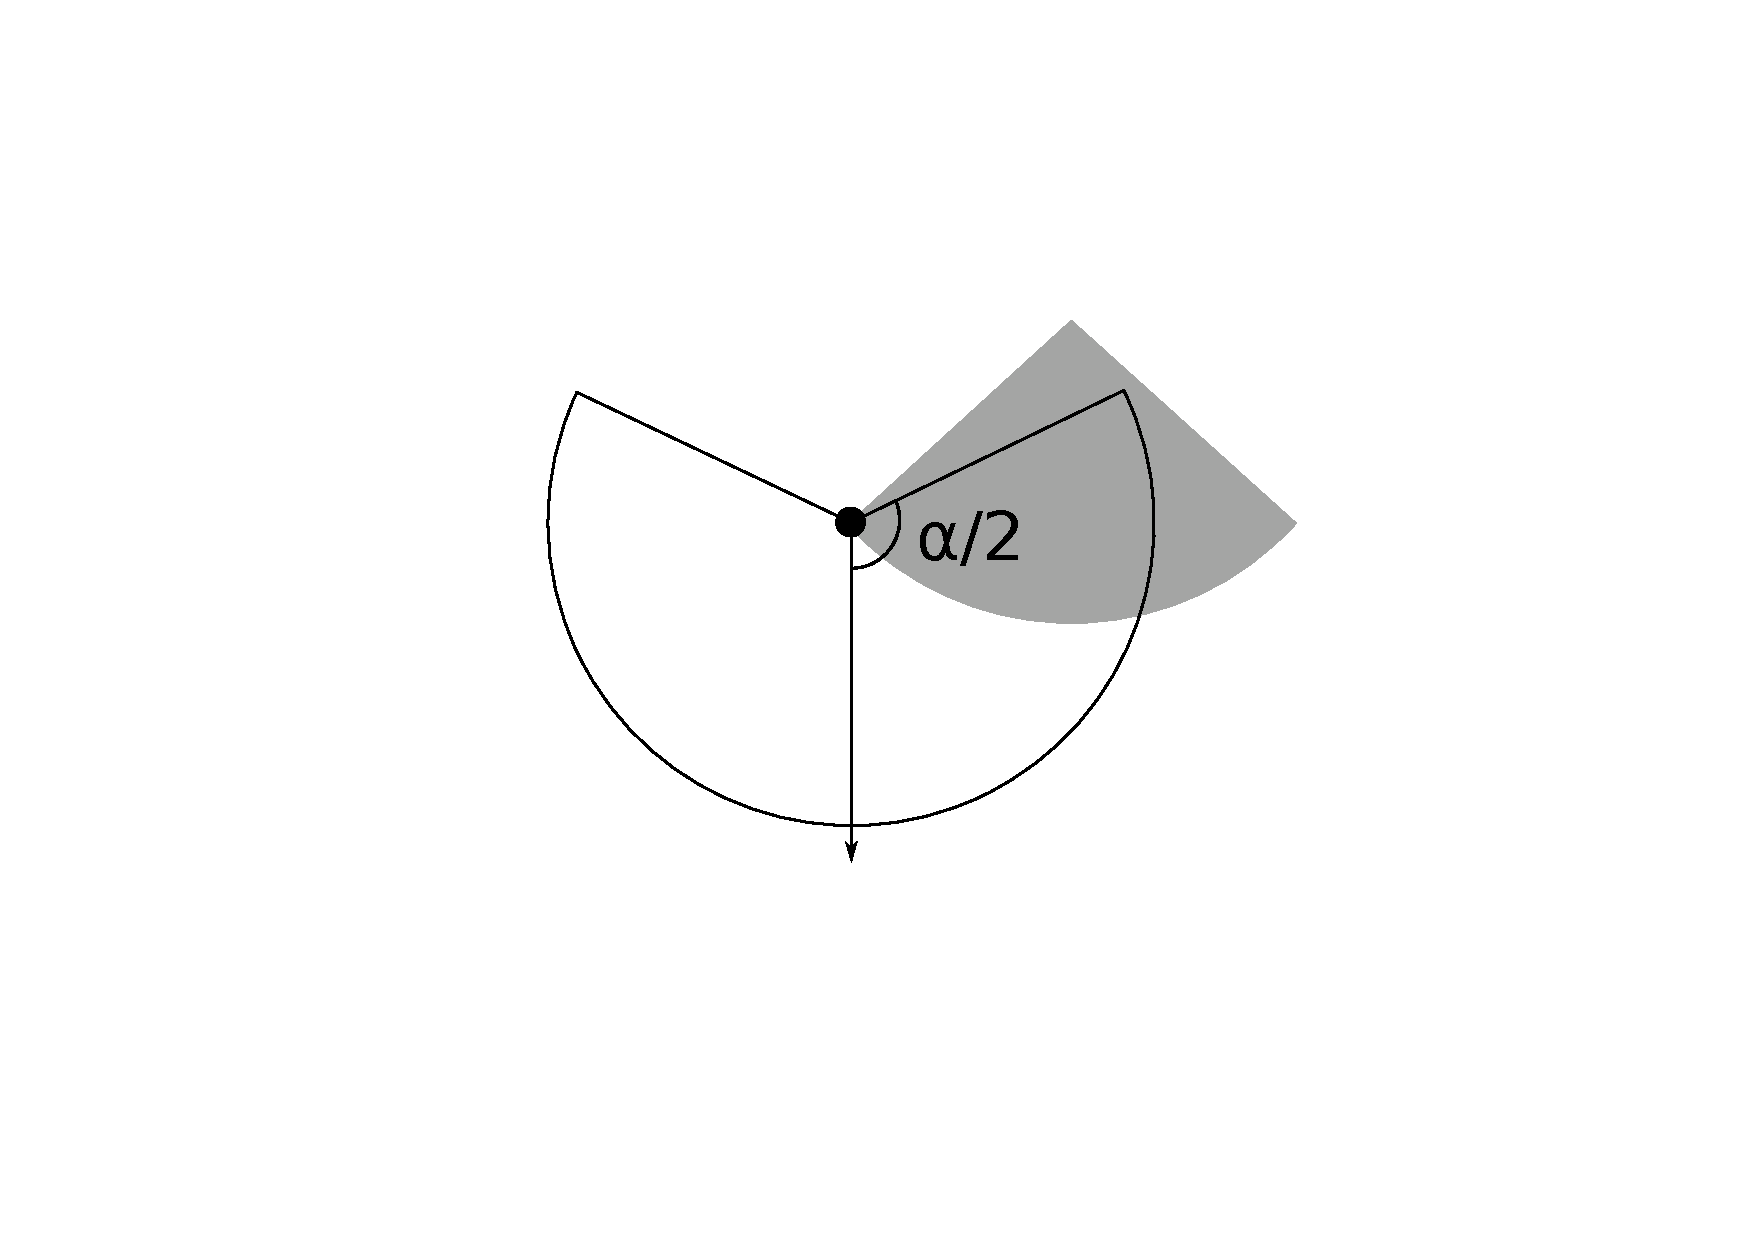
\includegraphics[width=1\textwidth, trim=5cm 6cm 4cm 1cm]{imgs/behind.pdf}
                \label{f:NW2--4behind}
                \caption{}
        \end{subfigure}
~ 
        \begin{subfigure}[t]{0.35\textwidth}
                \centering
        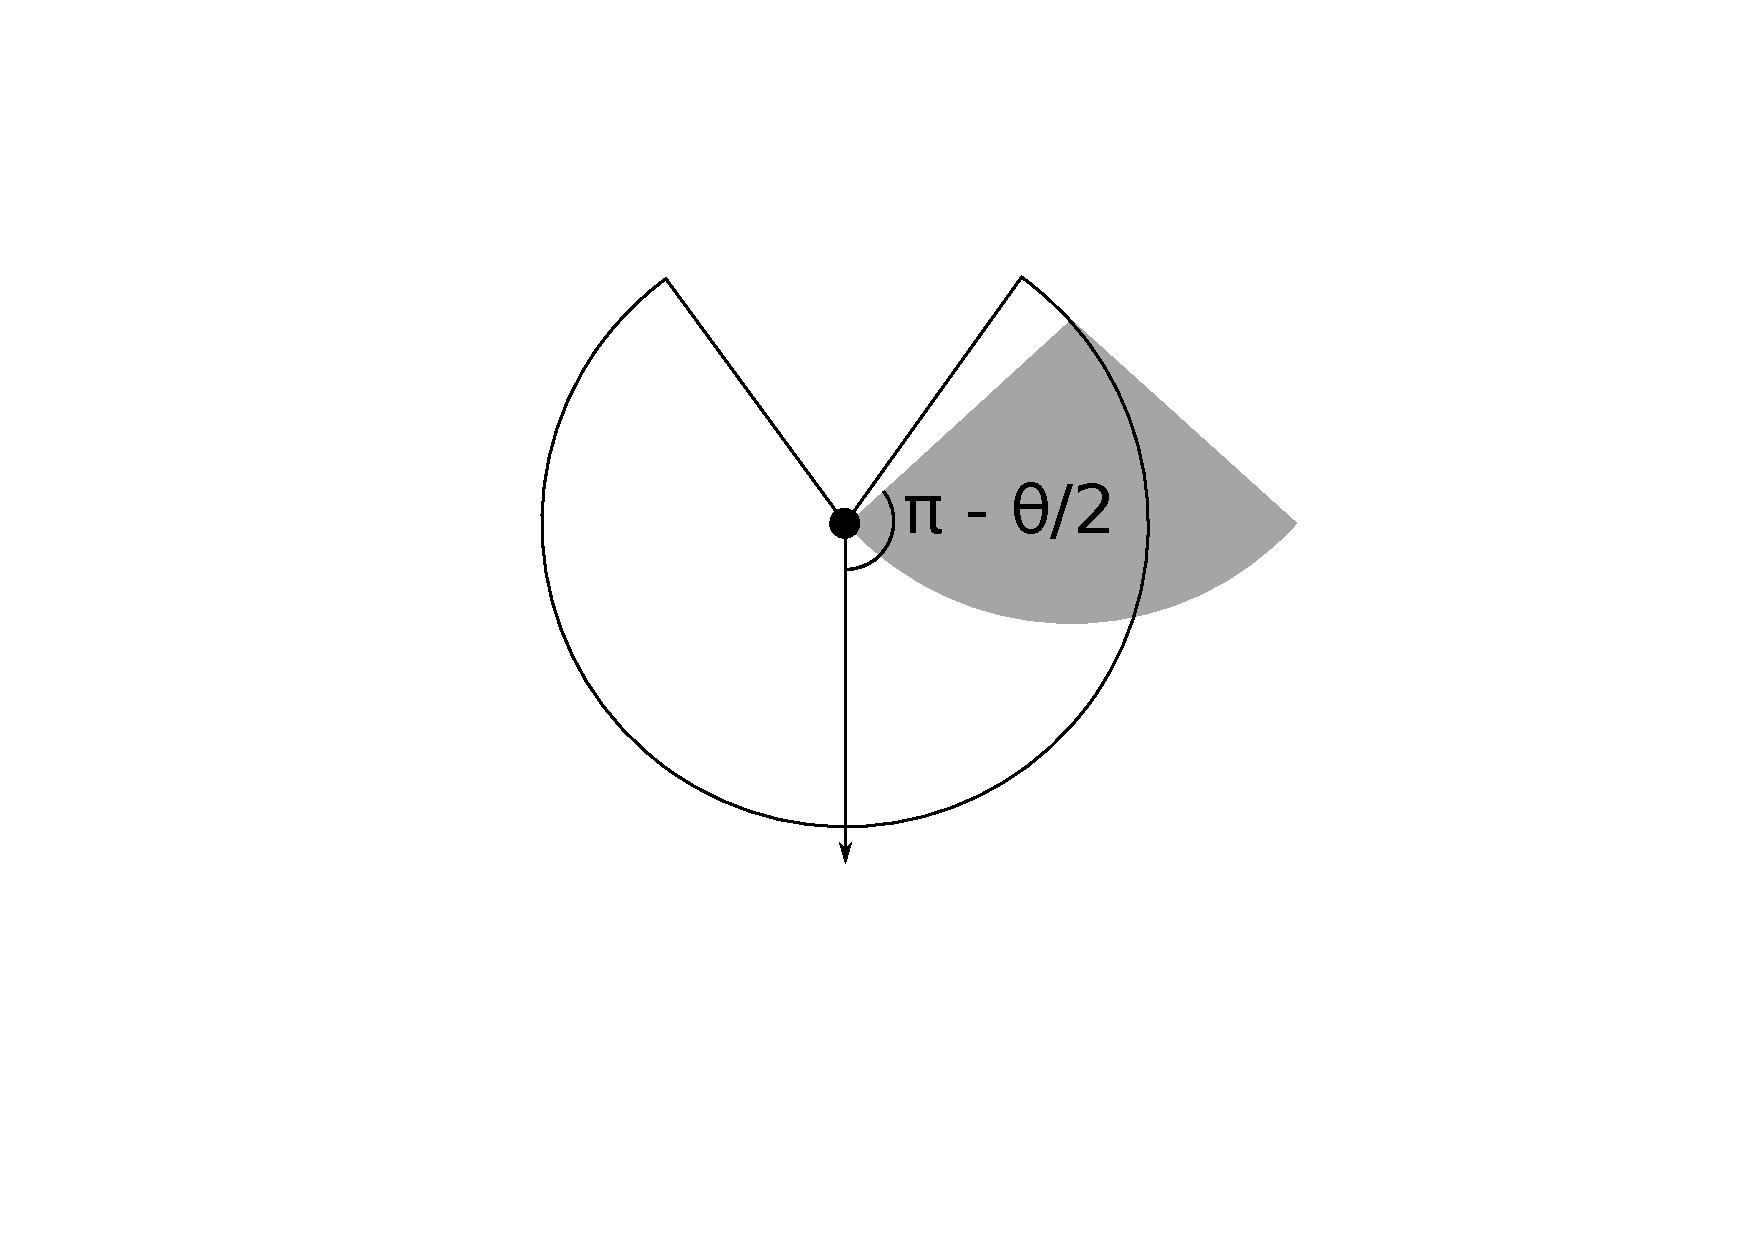
\includegraphics[width=1\textwidth, trim=5cm 6cm 4cm 1cm]{imgs/behind2.pdf}
                \label{f:NW2--4behind2}
                \caption{}
        \end{subfigure}

\caption{A) If $\alpha/2$ is less than $\pi - \theta/2$, as is the case here, then the width of the profile when an animal approaches directly from behind is zero. B) If $\alpha/2 > \pi - \theta/2$ the profile width from behind is $2r\sin\left(\frac{\theta}{2}\right)\sin(x_2)$.}
\label{f:NW2--4}
\end{figure}


\subsubsection{Model NW2} \label{NW2}

NW2 is bounded by $\alpha \ge 3\pi - 2\theta$, $\alpha \le 2\pi$ and $\theta\le\pi$.

NW2 has all five profiles as found in NW1. However, the change from the $r$ profile (third integral) to the $r - r\cos(x_4)$ profile (fourth integral) occurs at $x_4 = 3\pi/2 - \alpha/2$ instead of at $x_4 = \theta$. 

\begin{align}
    \mathrm{pNW2} =&\frac{1}{\pi} \left(\;\;\int\limits_{\frac{\theta}{2}}^{\frac{\pi}{2}}2 r \sin{\left (\frac{\theta}{2} \right )} \sin{\left (x_{2} \right )}\;\mathrm{d}x_{2}+\int\limits_{0}^{- \frac{\pi}{2} + \theta}r - r \cos{\left (- x_{4} + \theta \right )}\;\mathrm{d}x_{4}\right.\notag\\
 &\left.+\int\limits_{- \frac{\pi}{2} + \theta}^{\frac{3 \pi}{2} - \frac{\alpha}{2}}r\;\mathrm{d}x_{4}+\int\limits_{\frac{3 \pi}{2} - \frac{\alpha}{2}}^{\theta}r - r \cos{\left (x_{4} \right )}\;\mathrm{d}x_{4}+\int\limits_{\frac{\theta}{2}}^{\frac{\pi}{2}}2 r \sin{\left (\frac{\theta}{2} \right )} \sin{\left (x_{2} \right )}\;\mathrm{d}x_{2}\right)\label{pNW2Def}\\
    \mathrm{pNW2} =& \frac{r}{\pi} \left(\theta - \cos{\left (\frac{\alpha}{2} \right )} + 1\right)\label{pNW2Sln}
\end{align}


\subsubsection{Model NW3} \label{NW3}

NW3 is bounded by $\alpha \le 3\pi - 2\theta$, $\alpha\ge 2\pi-\theta$ and $\theta\ge\pi/2$.

NW3 does not have the fourth integral from NW2 as the right side of the profile does not become viable until after the $x_4$ region has ended and the $x_2$ region has begun. Therefore the second $x_4$ integral has an upper limit of $\theta $ and the integral after has a width of $r\cos(x_2 - \theta/2)$ and is integrated with respect to $x_2$. The final integral starts at $x_4 = 3\pi/2 - \alpha/2 - \theta/2$ and has the full width of $2r\sin(x_2)\sin(\theta/2)$.

\begin{align}
    \mathrm{pNW3} =&\frac{1}{\pi} \left(\;\;\int\limits_{\frac{\theta}{2}}^{\frac{\pi}{2}}2 r \sin{\left (\frac{\theta}{2} \right )} \sin{\left (x_{2} \right )}\;\mathrm{d}x_{2}+\int\limits_{0}^{- \frac{\pi}{2} + \theta}r - r \cos{\left (- x_{4} + \theta \right )}\;\mathrm{d}x_{4}\right.\notag\\
 &\left.+\int\limits_{- \frac{\pi}{2} + \theta}^{\theta}r\;\mathrm{d}x_{4}+\int\limits_{\frac{\theta}{2}}^{\frac{3 \pi}{2} - \frac{\theta}{2} - \frac{\alpha}{2}}r \cos{\left (- x_{2} + \frac{\theta}{2} \right )}\;\mathrm{d}x_{2}+\int\limits_{\frac{3 \pi}{2} - \frac{\theta}{2} - \frac{\alpha}{2}}^{\frac{\pi}{2}}2 r \sin{\left (\frac{\theta}{2} \right )} \sin{\left (x_{2} \right )}\;\mathrm{d}x_{2}\right)\label{pNW3Def}\\
    \mathrm{pNW3} =& \frac{r}{\pi} \left(\theta - \cos{\left (\frac{\alpha}{2} \right )} + 1\right)\label{pNW3Sln}
\end{align}

\subsubsection{Model NW4} \label{NW4}

Finally, NW4 is bounded by $\alpha\ge \pi$, $\theta\ge \pi/2$ and $\alpha \le 2\pi - \theta$. NW4 is the same as NW3 except that the final profile width is zero and this profile is reached at $\alpha/2+\theta/2-\pi/2$. 

\begin{align}
    \bar{p}_{\text{\tiny{NW4}}} =&\frac{1}{\pi} \left(\;\;\int\limits_{\frac{\theta}{2}}^{\frac{\pi}{2}}2 r \sin{\left (\frac{\theta}{2} \right )} \sin{\left (x_{2} \right )}\;\mathrm{d}x_{2}+\int\limits_{0}^{\theta - \frac{\pi}{2}}r - r \cos{\left (- x_{4} + \theta \right )}\;\mathrm{d}x_{4}\right.\notag\\
 &\left.+\int\limits_{\theta - \frac{\pi}{2}}^{\theta}r\;\mathrm{d}x_{4}+\int\limits_{\frac{\theta}{2}}^{\frac{\alpha}{2} + \frac{\theta}{2} - \frac{\pi}{2}}r \cos{\left (\frac{\theta}{2} - x_{2} \right )}\;\mathrm{d}x_{2}\right)\label{pNW4Def}\\
    \bar{p}_{\text{\tiny{NW4}}}  =& \frac{r}{\pi} \left(\theta - \cos{\left (\frac{\alpha}{2} \right )} + 1\right)\label{pNW4Sln}
\end{align}


\subsection{Model REM} \label{REM}

REM is the model from \citep{rowcliffe2008estimating}. It has $\alpha =2\pi$ and $\theta \le \pi/2$. It has three profile widths, two of which are repeated, once as the animal approaches from on front of the sensor and once as the animal approaches from behind the sensor.

\begin{enumerate}
\item Starting with an approach direction of directly towards the sensor, and examining focal angle $x_2$, the profile width is $2r\sin(x_2)\sin(\theta/2)$. 
\item When the profile is perpendicular to the radius edge of the sector sensor region, we instead examine $x_3$ where the profile width is $r\sin(x_3)$.
\item At $x_3=\pi/2$ the profile becomes simply $r$ and this continues for $\theta $ radians of $x_4$. 
\item The $x_3$ profile is then repeated with an approach direction from behind the sensor. 
\item Finally the $x_2$ profile is repeated, again with an approach direction from behind the sensor. 
\end{enumerate}

\begin{align}
    \mathrm{pREM} =&\frac{1}{\pi} \left(\;\;\int\limits_{\frac{\pi}{2} - \frac{\theta}{2}}^{\frac{\pi}{2}}2 r \sin{\left (\frac{\theta}{2} \right )} \sin{\left (x_{2} \right )}\;\mathrm{d}x_{2}+\int\limits_{\theta}^{\frac{\pi}{2}}r \sin{\left (x_{3} \right )}\;\mathrm{d}x_{3}\right.\notag\\
 &\left.+\int\limits_{0}^{\theta}r\;\mathrm{d}x_{4}+\int\limits_{\theta}^{\frac{\pi}{2}}r \sin{\left (x_{3} \right )}\;\mathrm{d}x_{3}+\int\limits_{\frac{\pi}{2} - \frac{\theta}{2}}^{\frac{\pi}{2}}2 r \sin{\left (\frac{\theta}{2} \right )} \sin{\left (x_{2} \right )}\;\mathrm{d}x_{2}\right)\label{pREMDef}\\
    \mathrm{pREM} =& \frac{r}{\pi} \left(\theta + 2\right)\label{pREMSln}
\end{align}

\subsection{Model NW5--7} \label{NW57}

In the models in NW5--7, the sensor has $\theta \le \pi/2$ as in the REM. As $\alpha \ge \pi/2$ a lot of the profiles are similar to the REM. Specifically, the first three profiles are always the same as the first three profiles of the REM. This is because when an animal is moving towards the sensor, the $\alpha \ge \pi$ call is no different to a $2\pi$ call. However, when approaching the sensor from behind, things are slightly different. The animal can only be detected by the sensor if the signal width is large enough that it can be detected once it has passed the sensor. 
                    
\begin{enumerate}
\item Starting with an approach direction of directly towards the sensor, and examining focal angle $x_2$, the profile width is $2r\sin(x_2)\sin(\theta/2)$. 
\item When the profile is perpendicular to the radius edge of the sector sensor region, we instead examine $x_3$ where the profile width is $r\sin(x_3)$.
\item At $x_3=\pi/2$ the profile becomes simply $r$ and this continues for $\theta $ radians of $x_4$. 
\item If $\alpha \le 2\pi + 2\theta$, the animal becomes undetectable during this profile when  $x_3$ has decreased in size to $\pi - \alpha/2$. This inequality marks the boundary between NW7 and NW6. 
\item If instead $\alpha \ge 2\pi + 2\theta$ then the animal does not become undetectable during the $x_3$ focal angle. Instead the profile has width greater than zero for the whole of the $x_3$ angle and the the second $x_2$ angle is reached. The profile starts with width $r\cos(x_2 - \theta/2)$ as only animals approaching to the left of the sensor are detectable. 
\item During this second $x_2$ profile the call angle needed for animals to be detected to the left of the detector is increasing while the angle needed for animals to be detected to the right of the detector is decreasing. Therefore, either the left side becomes undetectable, making both sides undetectable (this occurs if $\alpha \le 2\pi - \theta$ as in NW6) \item or the right becomes detectable (if $\alpha \ge 2\pi - \theta$ as in NW5), making both sides detectable and giving a profile width of $2r\sin(x_2)\sin(\theta/2)$.
\end{enumerate}


\subsubsection{Model NW5} \label{NW5}

NW5 is bounded by $\alpha \ge 2\pi - \theta$, $\alpha \le 2\pi$ and $\theta \le \pi/2$.

It is the same as REM except that it includes the extra profile in $x_2$ (the fifth integral) where only animals approaching to the left of the profile are detected.

\begin{align}
    \bar{p}_{\text{\tiny{NW5}}} =&\frac{1}{\pi} \left(\;\;\int\limits_{\frac{\pi}{2} - \frac{\theta}{2}}^{\frac{\pi}{2}}2 r \sin{\left (\frac{\theta}{2} \right )} \sin{\left (x_{2} \right )}\;\mathrm{d}x_{2}+\int\limits_{\theta}^{\frac{\pi}{2}}r \sin{\left (x_{3} \right )}\;\mathrm{d}x_{3}+\int\limits_{0}^{\theta}r\;\mathrm{d}x_{4}\right.\notag\\
 &\left.+\int\limits_{\theta}^{\frac{\pi}{2}}r \sin{\left (x_{3} \right )}\;\mathrm{d}x_{3}+\int\limits_{\frac{\pi}{2} - \frac{\theta}{2}}^{\frac{3 \pi}{2} - \frac{\theta}{2} - \frac{\alpha}{2}}r \cos{\left (\frac{\theta}{2} - x_{2} \right )}\;\mathrm{d}x_{2}+\int\limits_{\frac{3 \pi}{2} - \frac{\theta}{2} - \frac{\alpha}{2}}^{\frac{\pi}{2}}2 r \sin{\left (\frac{\theta}{2} \right )} \sin{\left (x_{2} \right )}\;\mathrm{d}x_{2}\right)\label{pNW5Def}\\
    \bar{p}_{\text{\tiny{NW5}}}  =& \frac{r}{\pi} \left(\theta - \cos{\left (\frac{\alpha}{2} \right )} + 1\right)\label{pNW5Sln}
\end{align}

\subsubsection{Model NW6} \label{NW6}

NW6 is bounded by $\alpha \le 2\pi - \theta$, $\alpha \ge 2\pi + 2\theta$ and $\theta \le \pi/2$

NW6 is the same NW5 except that as $\alpha \le 2\pi - \theta$, animals that approach from directly behind the detector are not detected. Therefore at $x_2 = \alpha/2 + \theta/2 - \pi/2$ the profile width goes to zero and therefore the last integral in NW5 is not included.

\begin{align}
    \bar{p}_{\text{\tiny{NW6}}} =&\frac{1}{\pi} \left(\;\;\int\limits_{\frac{\pi}{2} - \frac{\theta}{2}}^{\frac{\pi}{2}}2 r \sin{\left (\frac{\theta}{2} \right )} \sin{\left (x_{2} \right )}\;\mathrm{d}x_{2}+\int\limits_{\theta}^{\frac{\pi}{2}}r \sin{\left (x_{3} \right )}\;\mathrm{d}x_{3}\right.\notag\\
 &\left.+\int\limits_{0}^{\theta}r\;\mathrm{d}x_{4}+\int\limits_{\theta}^{\frac{\pi}{2}}r \sin{\left (x_{3} \right )}\;\mathrm{d}x_{3}+\int\limits_{\frac{\pi}{2} - \frac{\theta}{2}}^{\frac{\alpha}{2} + \frac{\theta}{2} - \frac{\pi}{2}}r \cos{\left (\frac{\theta}{2} - x_{2} \right )}\;\mathrm{d}x_{2}\right)\label{pNW6Def}\\
    \bar{p}_{\text{\tiny{NW6}}}  =& \frac{r}{\pi} \left(\theta - \cos{\left (\frac{\alpha}{2} \right )} + 1\right)\label{pNW6Sln}
\end{align}



\subsubsection{Model NW7} \label{NW7}

NW7 is bounded by $\alpha \ge 2\pi + 2\theta$, $\alpha \ge \pi$ and $\theta \ge 0$.

It is similar to NW6 but does not include the last integral as during the $x_3$ profile, at $x_3 = \pi - \alpha/2$ the call width is too small for any animals to be detected, so the profile width goes to zero.

\begin{align}
    \mathrm{pNW7} =&\frac{1}{\pi} \left(\;\;\int\limits_{\frac{\pi}{2} - \frac{\theta}{2}}^{\frac{\pi}{2}}2 r \sin{\left (\frac{\theta}{2} \right )} \sin{\left (x_{2} \right )}\;\mathrm{d}x_{2}+\int\limits_{\theta}^{\frac{\pi}{2}}r \sin{\left (x_{3} \right )}\;\mathrm{d}x_{3}\right.\notag\\
 &\left.+\int\limits_{0}^{\theta}r\;\mathrm{d}x_{4}+\int\limits_{\pi - \frac{\alpha}{2}}^{\frac{\pi}{2}}r \sin{\left (x_{3} \right )}\;\mathrm{d}x_{3}\right)\label{pNW7Def}\\
    \mathrm{pNW7} =& \frac{r}{\pi} \left(\theta - \cos{\left (\frac{\alpha}{2} \right )} + 1\right)\label{pNW7Sln}
\end{align}





\subsection{Model SW1--3} \label{SW13}
 
The models in SW1--3 are described with the two focal angles used in models NW2--4, $x_2$ and $x_4$. As $\alpha \le\pi$ an animal can never be detected if it is approaching the detector from behind. This makes these models simpler in that they go through the $x_2$ and $x_4$ profiles only once each. 

\begin{figure}[t]
        \centering
        \begin{subfigure}[t]{0.35\textwidth}
                \centering
        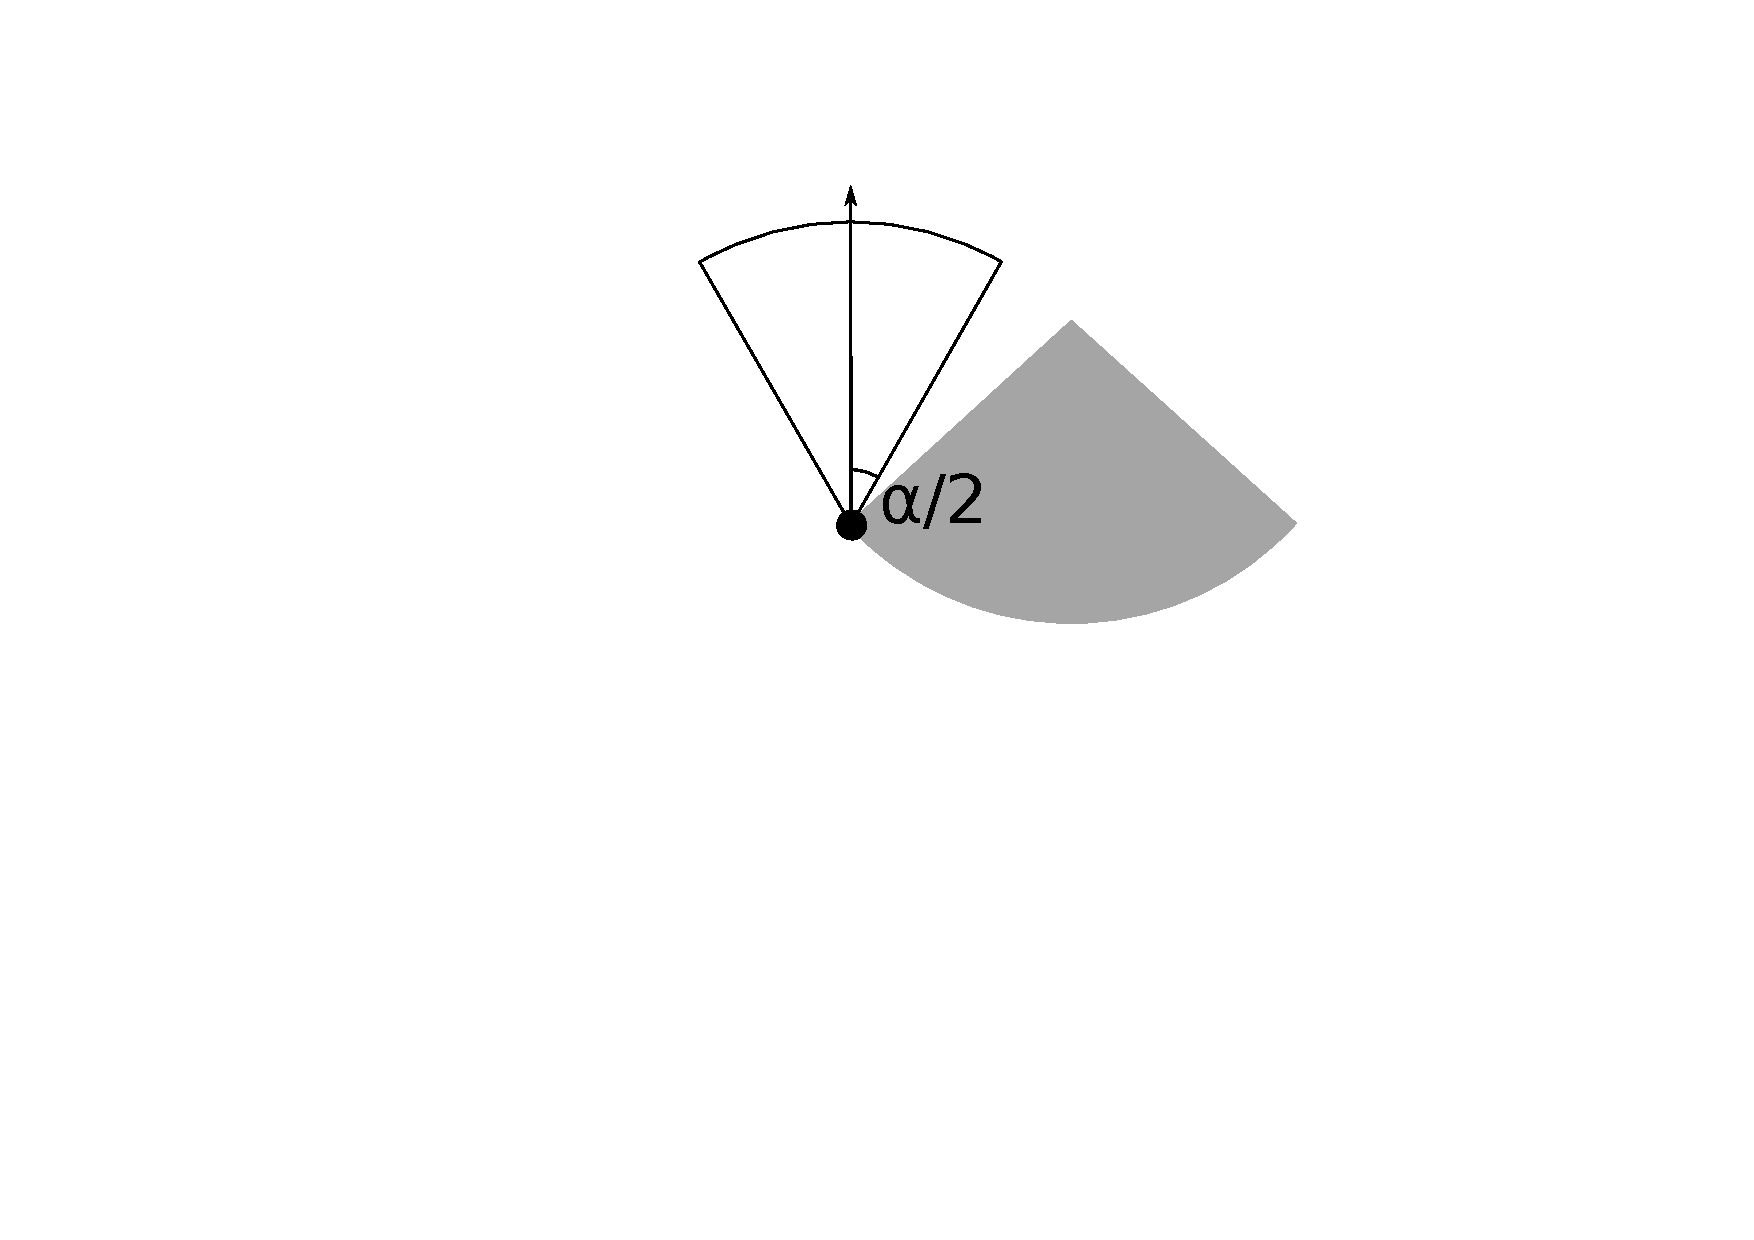
\includegraphics[width=1\textwidth, trim=7cm 10cm 6cm 1cm]{imgs/forward.pdf}
                \caption{}
                \label{f:SWforward} %NW1AT
        \end{subfigure}
~ 
        \begin{subfigure}[t]{0.35\textwidth}
                \centering
        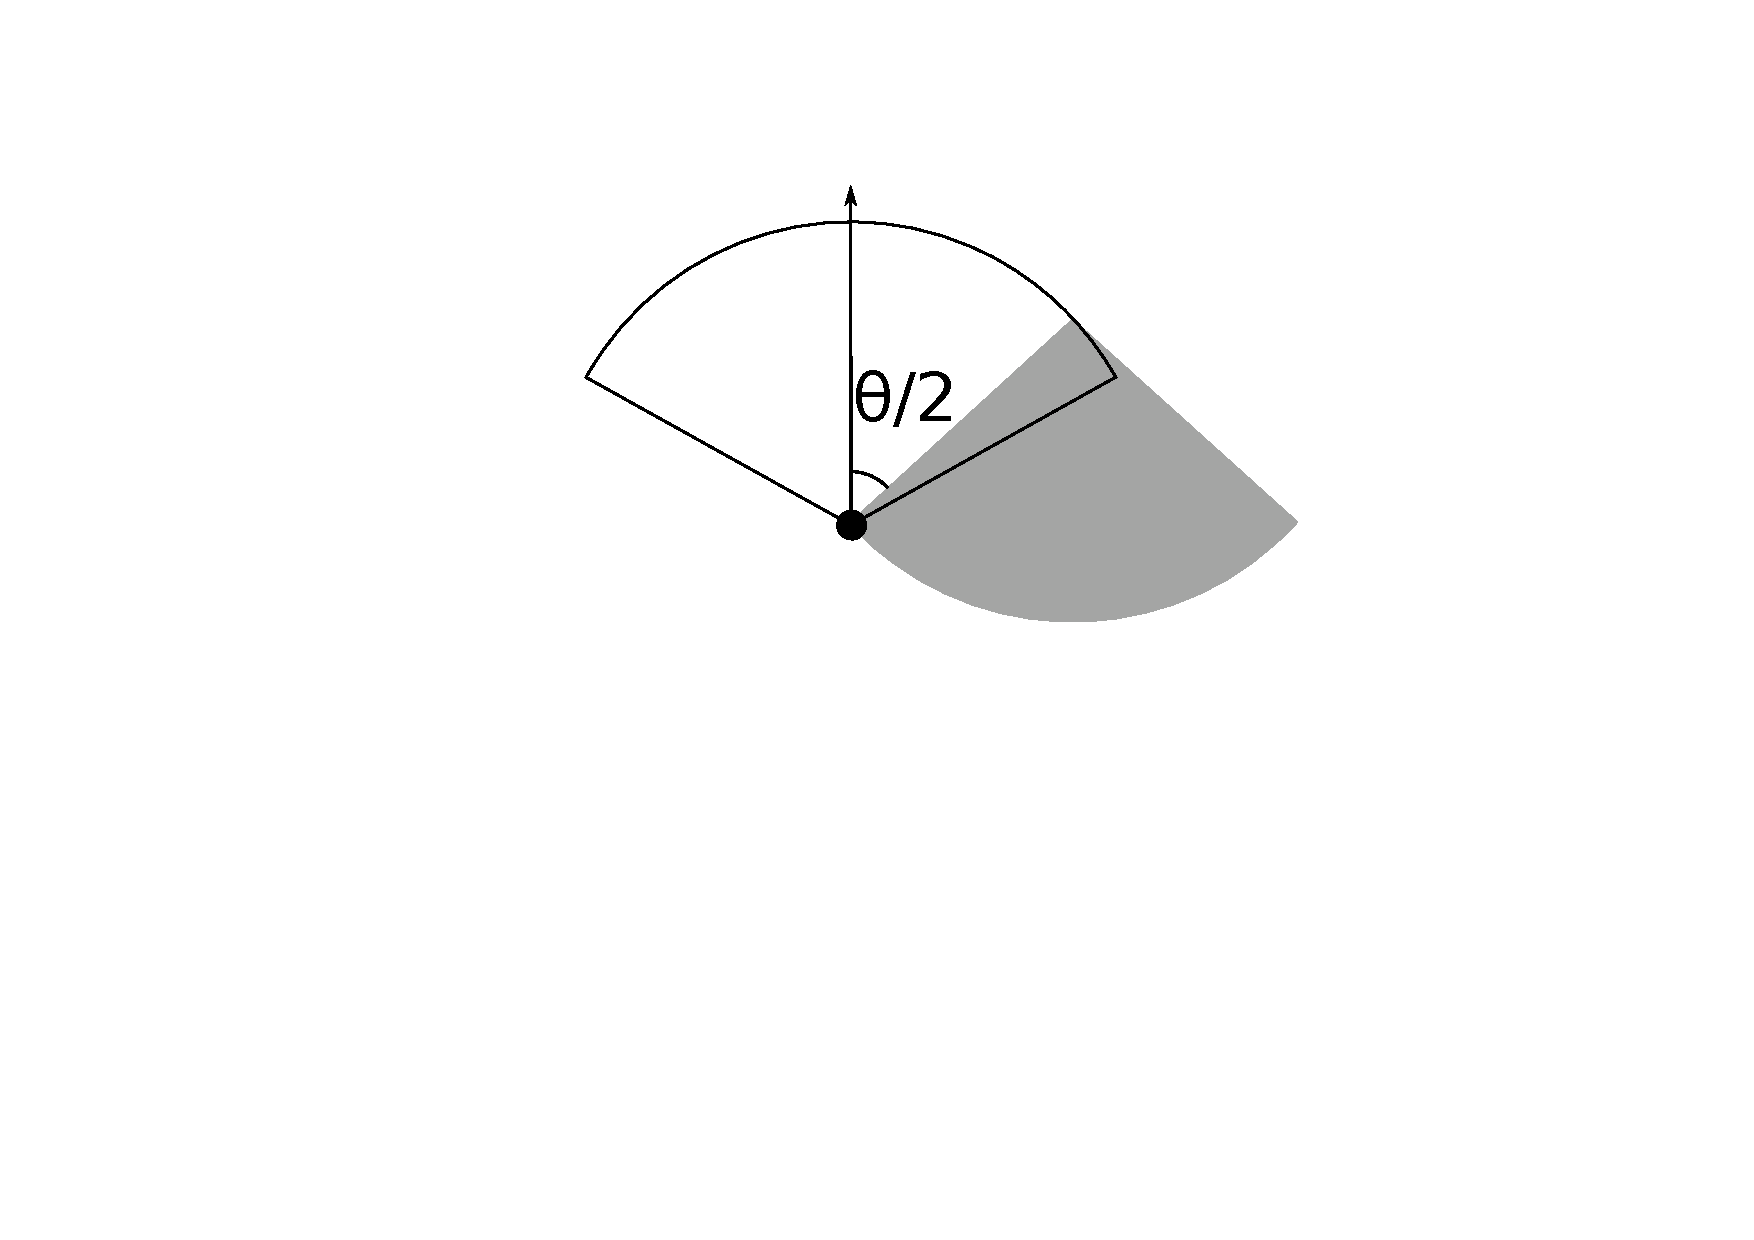
\includegraphics[width=1\textwidth, trim=7cm 10cm 6cm 1cm]{imgs/forward2.pdf}
                \caption{}
                \label{f:SWforwad2}
        \end{subfigure}

\caption{A)  As $\alpha/2 < \theta/2$ the profile width is limited by the call angle rather than the sensor region. The profile width is $2r\sin\left(\frac{\alpha}{2}\right)$ B) As $\alpha/2 > \theta/2$ the profile width is limited by the sensor region, not the call angle. The profile width is $2r\sin\left(\frac{\theta}{2}\right)\sin(x_2)$.    }
\label{f:forward}
\end{figure}


There are five potential profile sizes. 
\begin{enumerate}
\item At the beginning of $x_2$, with an approach direction directly towards the sensor, the parameter that limits the width of the profile can either be the sensor width,  in which case the profile width is $2r\sin\left(\theta/2\right)\sin(x_2)$. 
\item Or the call width can be the limiting parameter, in which case the profile width is instead $2r\sin(\alpha /2)$ (see Fig.~\ref{f:forward})
\item The next potential profile in $x_2$ has a width of $r\sin(\alpha/2) - r\cos(x_2 + \theta/2)$ as the right side of the profile is limited by the width of the sensor region while the left side is limited by the call width. However, the angle at which the profile starts depends on whether the first profile was 1) or 2) above. If the first profile is profile 1) then the profile is limited on both sides by the sensor region and then the left side of the profile becomes limited by the call width. This happens at $x_2 = \pi/2 - \alpha/2 + \theta/2$. If however the first profile was 2) then the first profile is limited by the call width. We move into the new profile when the right side of the profile becomes limited by the sensor region. This occurs at $x_2 = \pi/2 + \alpha/2 - \theta/2$.


\item In the $x_4$ region the left side of the profile is always $r\sin(\alpha /2)$ while the right side is either 0, giving a profile of $r\sin(\alpha /2)$. 

\item Or limited by the sensor giving a profile of size $r\sin (\alpha /2) -r\cos(x_4-\theta) $.
\end{enumerate}

\subsubsection{Model SW1} \label{SW1}

SW1 is bounded by $\alpha \ge \theta$, $\alpha \le\pi$ and $\theta \le \pi$.

As $\alpha $ is large the first profile is limited by the size of the sensor region giving it a width of $2r\sin\left(\theta/2\right)\sin(x_2)$. It is the only one of the three SW models to start in this way. Later on, still with $x_2$ as the focal angle the left side of the profile does become limited by the call width. So at $x_2= \pi/2 - \alpha/2 + \theta/2$ the profile width becomes $r\sin(\alpha/2) - r\cos(x_2 + \theta/2)$. 

As we enter the $x_4$ region, the profile remains limited by the call on the left and by the sensor on the right, giving a profile width of  $r\sin (\alpha /2) -r\cos(x_4-\theta) $. Finally, at $x_4 = \theta - \pi/2$ the right side of the profile becomes zero and the profile is width is $r\sin(\alpha /2)$.

\begin{align}
    \mathrm{pSW1} =&\frac{1}{\pi} \left(\;\;\int\limits_{\frac{\pi}{2} + \frac{\theta}{2} - \frac{\alpha}{2}}^{\frac{\pi}{2}}2 r \sin{\left (\frac{\theta}{2} \right )} \sin{\left (x_{2} \right )}\;\mathrm{d}x_{2}+\int\limits_{\frac{\theta}{2}}^{\frac{\pi}{2} + \frac{\theta}{2} - \frac{\alpha}{2}}- r \cos{\left (x_{2} + \frac{\theta}{2} \right )} + r \sin{\left (\frac{\alpha}{2} \right )}\;\mathrm{d}x_{2}\right.\notag\\
 &\left.+\int\limits_{0}^{- \frac{\pi}{2} + \theta}- r \cos{\left (- x_{4} + \theta \right )} + r \sin{\left (\frac{\alpha}{2} \right )}\;\mathrm{d}x_{4}+\int\limits_{- \frac{\pi}{2} + \theta}^{- \frac{\pi}{2} + \theta + \frac{\alpha}{2}}r \sin{\left (\frac{\alpha}{2} \right )}\;\mathrm{d}x_{4}\right)\label{pSW1Def}\\
    \mathrm{pSW1} =& \frac{r}{\pi} \left(\theta \sin{\left (\frac{\alpha}{2} \right )} - \cos{\left (\frac{\alpha}{2} \right )} + 1\right)\label{pSW1Sln}
\end{align}

\subsubsection{Model SW2} \label{SW2}

SW2 is bounded by $\theta \ge \pi/2$, $\alpha \le \theta$ and $\alpha \ge 2\theta -\pi$.

SW2 is largely similar to SW1. However, as $\alpha \le \theta$ the first profile is limited by $\alpha$ and not by the detection region. Therefore the first profile has width $2r\sin(\alpha /2)$. This also means the transition to the second profile occurs at  $x_2 = \pi/2 + \alpha/2 - \theta/2$ instead of  $x_2 = \pi/2 - \alpha/2 + \theta/2$.

\begin{align}
    \bar{p}_{\text{\tiny{SW2}}} =&\frac{1}{\pi} \left(\;\;\int\limits_{\frac{\alpha}{2} - \frac{\theta}{2} + \frac{\pi}{2}}^{\frac{\pi}{2}}2 r \sin{\left (\frac{\alpha}{2} \right )}\;\mathrm{d}x_{2}+\int\limits_{\frac{\theta}{2}}^{\frac{\alpha}{2} - \frac{\theta}{2} + \frac{\pi}{2}}r \sin{\left (\frac{\alpha}{2} \right )} - r \cos{\left (\frac{\theta}{2} + x_{2} \right )}\;\mathrm{d}x_{2}\right.\notag\\
 &\left.+\int\limits_{0}^{\theta - \frac{\pi}{2}}r \sin{\left (\frac{\alpha}{2} \right )} - r \cos{\left (\theta - x_{4} \right )}\;\mathrm{d}x_{4}+\int\limits_{\theta - \frac{\pi}{2}}^{\frac{\alpha}{2} + \theta - \frac{\pi}{2}}r \sin{\left (\frac{\alpha}{2} \right )}\;\mathrm{d}x_{4}\right)\label{pSW2Def}\\
    \bar{p}_{\text{\tiny{SW2}}}  =& \frac{r}{\pi} \left(\theta \sin{\left (\frac{\alpha}{2} \right )} - \cos{\left (\frac{\alpha}{2} \right )} + 1\right)\label{pSW2Sln}
\end{align}



\subsubsection{Model SW3} \label{SW3}

SW3 is bounded by $\alpha \le 2\theta -\pi$ and $\theta \le \pi$.

SW3 is similar to SW2 except that the profile does not become limited by sensor at all during the the $x_4$ regions. Therefore, at $x_4 = 0 $ the profile is still of width $2r\sin(\alpha /2)$. Only at $x_4 = \theta - \pi/2 - \alpha/2$ does the profile become limited on the right by the sensor region.

\begin{align}
    \mathrm{pSW3} =&\frac{1}{\pi} \left(\;\;\int\limits_{\frac{\theta}{2}}^{\frac{\pi}{2}}2 r \sin{\left (\frac{\alpha}{2} \right )}\;\mathrm{d}x_{2}+\int\limits_{0}^{- \frac{\pi}{2} + \theta - \frac{\alpha}{2}}2 r \sin{\left (\frac{\alpha}{2} \right )}\;\mathrm{d}x_{4}\right.\notag\\
 &\left.+\int\limits_{- \frac{\pi}{2} + \theta - \frac{\alpha}{2}}^{- \frac{\pi}{2} + \theta}- r \cos{\left (- x_{4} + \theta \right )} + r \sin{\left (\frac{\alpha}{2} \right )}\;\mathrm{d}x_{4}+\int\limits_{- \frac{\pi}{2} + \theta}^{- \frac{\pi}{2} + \theta + \frac{\alpha}{2}}r \sin{\left (\frac{\alpha}{2} \right )}\;\mathrm{d}x_{4}\right)\label{pSW3Def}\\
    \mathrm{pSW3} =& \frac{r}{\pi} \left(\theta \sin{\left (\frac{\alpha}{2} \right )} - \cos{\left (\frac{\alpha}{2} \right )} + 1\right)\label{pSW3Sln}
\end{align}


\subsection{Model SW4--9} \label{SW4--9}

As $\alpha < \pi$, animals approaching the sensor from behind can never be detected, so unlike REM, the second $x_2$ and $x_3$ profiles are always zero. The six models are split by three inequalities that relate to the models as follows.

\begin{enumerate}
\item Models with $\alpha \le \pi - 2\theta$  have no $x_4$ profile. This is because at $x_4 = 0$, the call angle is already too small to be detected as can be seen in Fig.~\ref{f:SW4--9nox4} where $\alpha/2 < \pi/2 - \theta$ which simplifies to give the previous inequality.

\item Models with $\alpha \le \theta$ are limited by $\alpha$ in the first, $x_2$ region (see Fig.~\ref{f:forward}), rather than being limited by $\theta$. Therefore this first profile is of width $2r\sin(\alpha/2)$ rather than $2r\sin(\theta/2)\sin(x_2)$.

\item Finally, models with $\alpha \le 2\theta$ have a second profile in $x_2$ where to one side of the sensor $\alpha$ is the limiting factor of profile width, while on the other side $\theta$ is (see Fig.~\ref{f:4--9int3}). This gives a width of $r\sin(\alpha/2) - r\cos(x_2 + \theta/2)$. This profile does not occur in models with $\alpha \ge 2\theta$.

\end{enumerate}

\begin{figure}[t]
       \centering
        \begin{subfigure}[t]{0.4\textwidth}
                \centering
        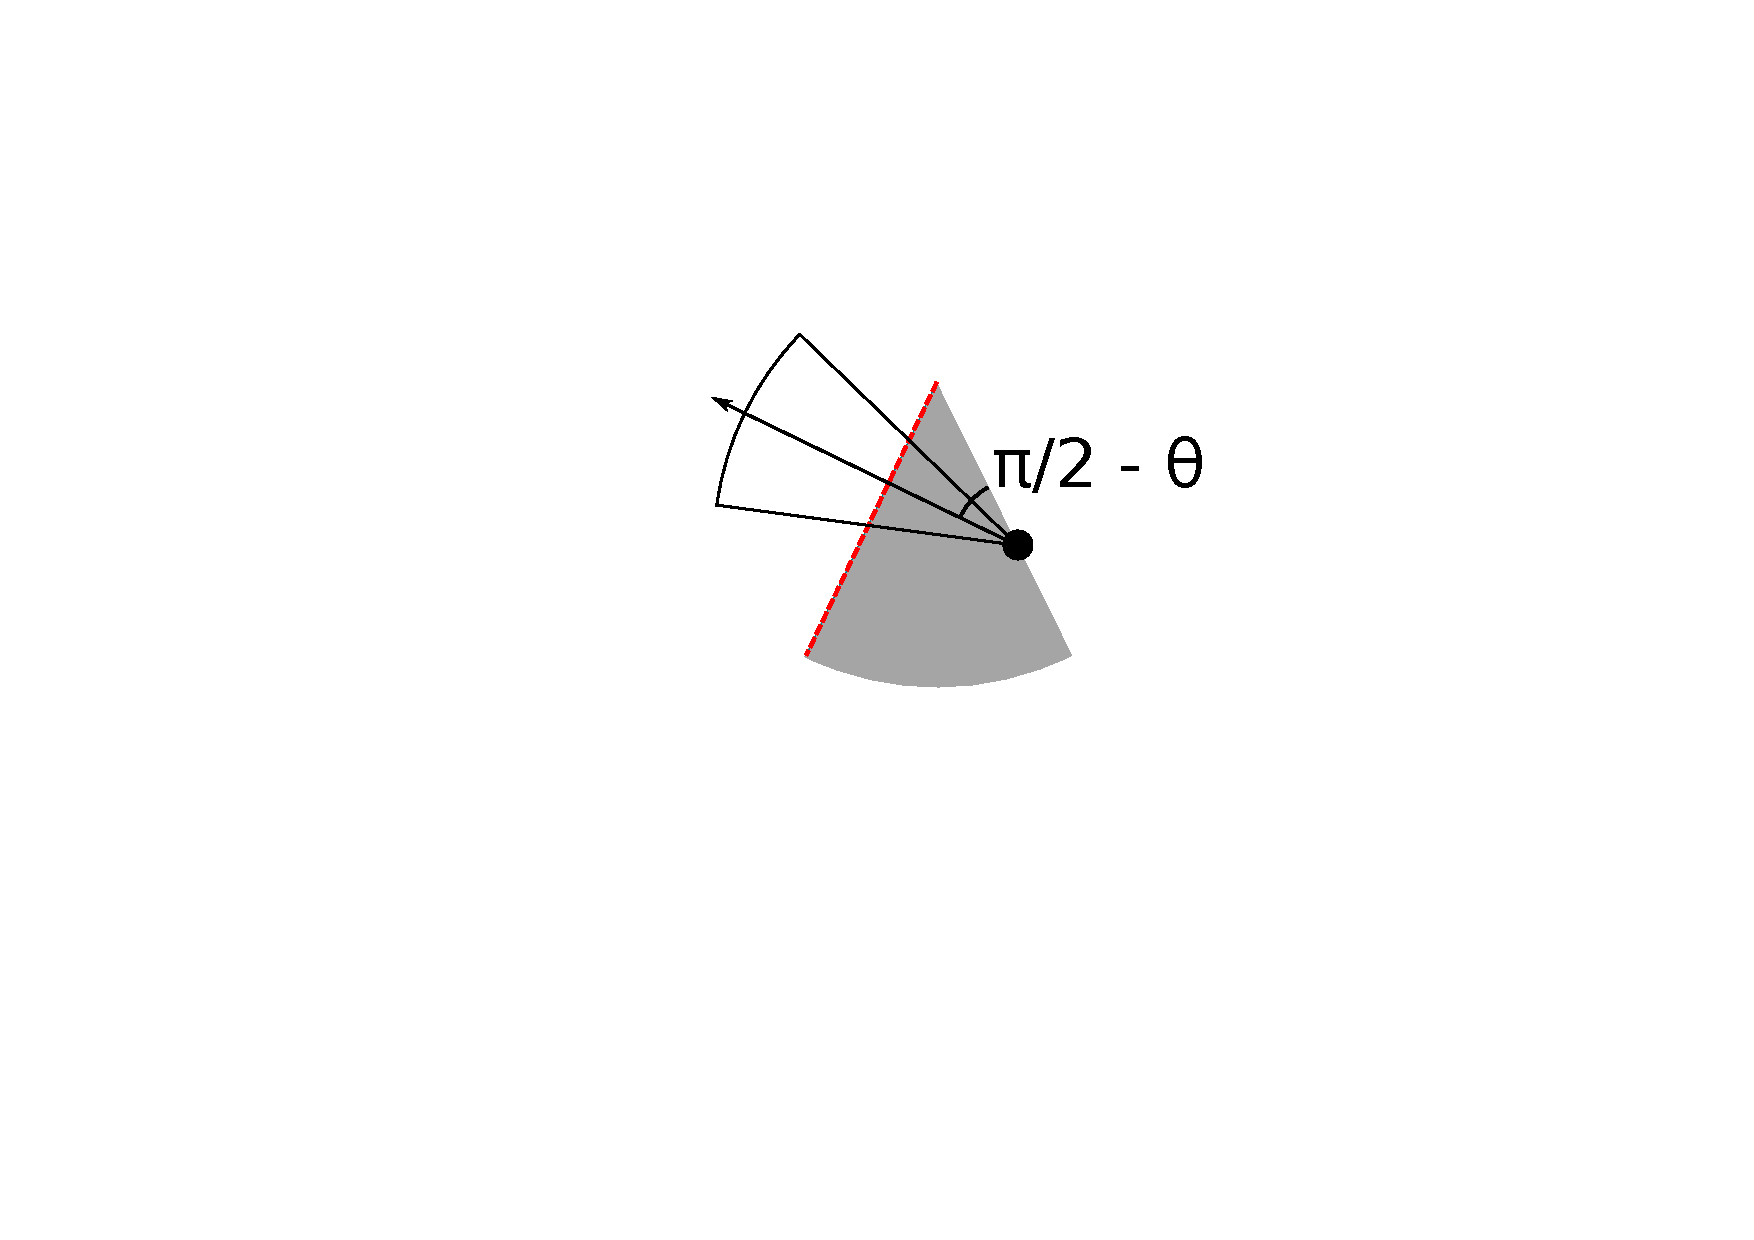
\includegraphics[width=1\textwidth, trim=8cm 9cm 8cm 4cm]{imgs/x4is0.pdf}
                \caption{}
                \label{f:SW4--9nox4}
        \end{subfigure}
~ 
        \begin{subfigure}[t]{0.4\textwidth}
                \centering
        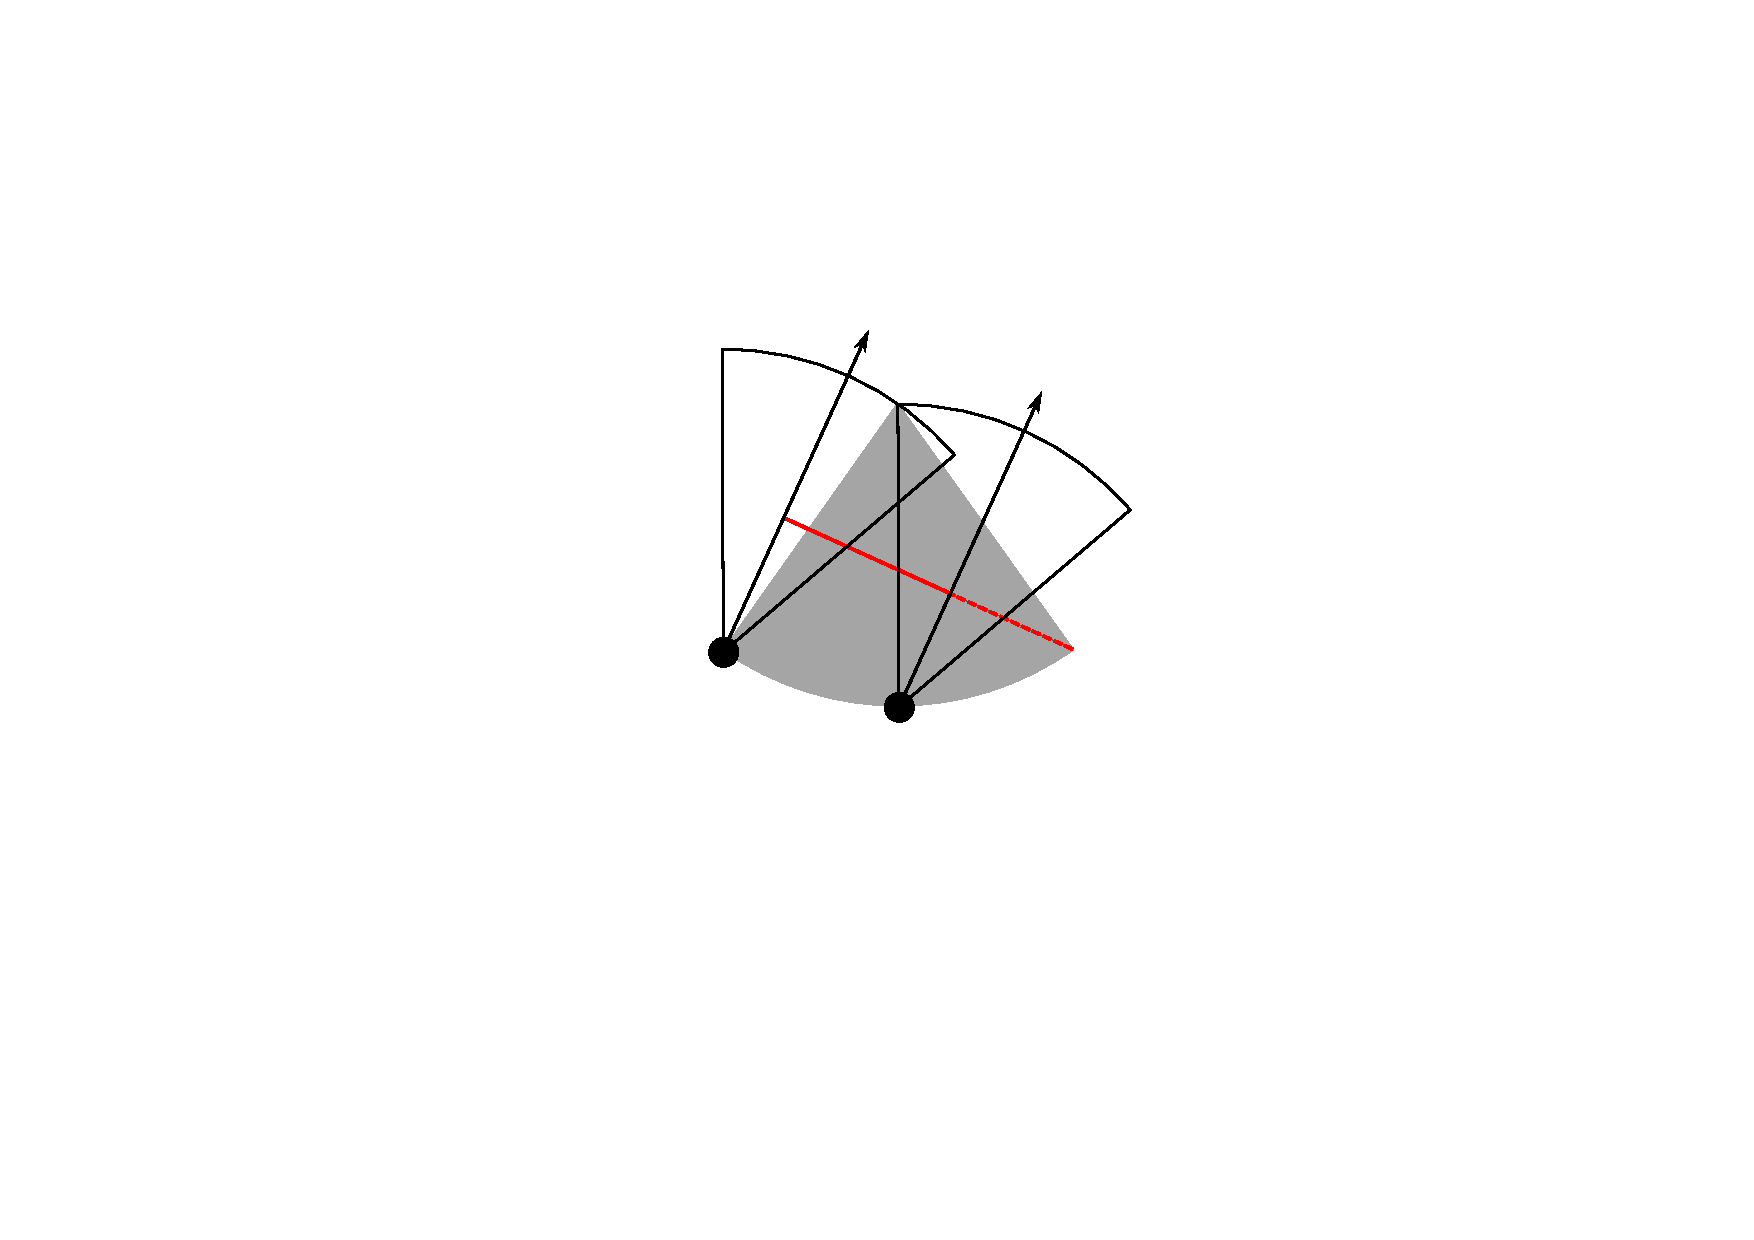
\includegraphics[width=1\textwidth, trim=8cm 9cm 8cm 4cm]{imgs/4--9int3.pdf}
                \caption{}
                \label{f:4--9int3}
        \end{subfigure}

\caption{A) At $x_4 = 0$, if $\alpha/2 < \pi/2 - \theta$ then $\alpha/2$ is too small for an animal to be detected at all during the $x_4$ profile (shown with dashed red.) This inequality simplifies to $\alpha < \pi - 2\theta$. B) The right of the profile is limited by the call width, not the sensor. On the left, the profile is limited by the sensor and not the call. Overall the profile width is $r\sin(\alpha/2) - r\cos(x_2 + \theta/2)$.     }
\label{f:SW4--9}
\end{figure}

\subsubsection{Model SW4} \label{SW4}

SW4 is bounded by $\alpha \le \theta$, $\alpha \ge \pi - 2\theta$ and $\theta \le \pi/2$. Therefore it does contain a $x_4$ profile, starts with an $\alpha$ limited profile and does contain the $r\sin(\alpha/2) - r\cos(x_2 + \theta/2)$ profile in $x_2$.

\begin{align}
    \mathrm{pSW4} =&\frac{1}{\pi} \left(\;\;\int\limits_{\frac{\pi}{2} - \frac{\theta}{2} + \frac{\alpha}{2}}^{\frac{\pi}{2}}2 r \sin{\left (\frac{\alpha}{2} \right )}\;\mathrm{d}x_{2}+\int\limits_{\frac{\pi}{2} - \frac{\theta}{2}}^{\frac{\pi}{2} - \frac{\theta}{2} + \frac{\alpha}{2}}- r \cos{\left (x_{2} + \frac{\theta}{2} \right )} + r \sin{\left (\frac{\alpha}{2} \right )}\;\mathrm{d}x_{2}\right.\notag\\
 &\left.+\int\limits_{\theta}^{\frac{\pi}{2}}r \sin{\left (\frac{\alpha}{2} \right )}\;\mathrm{d}x_{3}+\int\limits_{0}^{- \frac{\pi}{2} + \theta + \frac{\alpha}{2}}r \sin{\left (\frac{\alpha}{2} \right )}\;\mathrm{d}x_{4}\right)\label{pSW4Def}\\
    \mathrm{pSW4} =& \frac{r}{\pi} \left(\theta \sin{\left (\frac{\alpha}{2} \right )} - \cos{\left (\frac{\alpha}{2} \right )} + 1\right)\label{pSW4Sln}
\end{align}

\subsubsection{Model SW5} \label{SW5}

SW5 is the only model with a tetrahedral bounding region. It is bounded by $\alpha \ge \theta$, $\alpha \ge \pi - 2\theta$, $\alpha \le 2\theta$ and $\theta \le \pi/2$. Therefore it does contain a $x_4$ profile, but starts with a $\theta$ limited profile. It does contain the $r\sin(\alpha/2) - r\cos(x_2 + \theta/2)$ profile in $x_2$.

\begin{align}
    \bar{p}_{\text{\tiny{SW5}}} =&\frac{1}{\pi} \left(\;\;\int\limits_{\frac{\pi}{2} + \frac{\theta}{2} - \frac{\alpha}{2}}^{\frac{\pi}{2}}2 r \sin{\left (\frac{\theta}{2} \right )} \sin{\left (x_{2} \right )}\;\mathrm{d}x_{2}+\int\limits_{\frac{\pi}{2} - \frac{\theta}{2}}^{\frac{\pi}{2} + \frac{\theta}{2} - \frac{\alpha}{2}}r \sin{\left (\frac{\alpha}{2} \right )} - r \cos{\left (\frac{\theta}{2} + x_{2} \right )}\;\mathrm{d}x_{2}\right.\notag\\
 &\left.+\int\limits_{\theta}^{\frac{\pi}{2}}r \sin{\left (\frac{\alpha}{2} \right )}\;\mathrm{d}x_{3}+\int\limits_{0}^{\frac{\alpha}{2} + \theta - \frac{\pi}{2}}r \sin{\left (\frac{\alpha}{2} \right )}\;\mathrm{d}x_{4}\right)\label{pSW5Def}\\
    \bar{p}_{\text{\tiny{SW5}}}  =& \frac{r}{\pi} \left(\theta \sin{\left (\frac{\alpha}{2} \right )} - \cos{\left (\frac{\alpha}{2} \right )} + 1\right)\label{pSW5Sln}
\end{align}

\subsubsection{Model SW6} \label{SW6}

SW6 is bounded by $\alpha \ge \pi - 2\theta$,  $\alpha \ge 2\theta$ and $\alpha \le \pi$. It starts with a $\theta$ limeted profile and has a $x_4$ profile. However, it does not contain the $r\sin(\alpha/2) - r\cos(x_2 + \theta/2)$ profile.

\begin{align}
    \mathrm{pSW6} =&\frac{1}{\pi} \left(\;\;\int\limits_{\frac{\pi}{2} - \frac{\theta}{2}}^{\frac{\pi}{2}}2 r \sin{\left (\frac{\theta}{2} \right )} \sin{\left (x_{2} \right )}\;\mathrm{d}x_{2}+\int\limits_{\theta}^{\frac{\alpha}{2}}r \sin{\left (x_{3} \right )}\;\mathrm{d}x_{3}\right.\notag\\
 &\left.+\int\limits_{\frac{\alpha}{2}}^{\frac{\pi}{2}}r \sin{\left (\frac{\alpha}{2} \right )}\;\mathrm{d}x_{3}+\int\limits_{0}^{- \frac{\pi}{2} + \theta + \frac{\alpha}{2}}r \sin{\left (\frac{\alpha}{2} \right )}\;\mathrm{d}x_{4}\right)\label{pSW6Def}\\
    \mathrm{pSW6} =& \frac{r}{\pi} \left(\theta \sin{\left (\frac{\alpha}{2} \right )} - \cos{\left (\frac{\alpha}{2} \right )} + 1\right)\label{pSW6Sln}
\end{align}


\subsubsection{Model SW7} \label{SW7}

SW7 is bounded by $\alpha \le \pi - 2\theta$, $\alpha \le \theta$ and $\alpha < 0$. Therefore it does not contain a $x_4$ profile. It starts with an $\alpha$ limited profile and contains the $r\sin(\alpha/2) - r\cos(x_2 + \theta/2)$ profile in $x_2$.


\begin{align}
    \bar{p}_{\text{\tiny{SW7}}} =&\frac{1}{\pi} \left(\;\;\int\limits_{\frac{\alpha}{2} - \frac{\theta}{2} + \frac{\pi}{2}}^{\frac{\pi}{2}}2 r \sin{\left (\frac{\alpha}{2} \right )}\;\mathrm{d}x_{2}+\int\limits_{\frac{\pi}{2} - \frac{\theta}{2}}^{\frac{\alpha}{2} - \frac{\theta}{2} + \frac{\pi}{2}}r \sin{\left (\frac{\alpha}{2} \right )} - r \cos{\left (\frac{\theta}{2} + x_{2} \right )}\;\mathrm{d}x_{2}+\int\limits_{\theta}^{\frac{\alpha}{2} + \theta}r \sin{\left (\frac{\alpha}{2} \right )}\;\mathrm{d}x_{3}\right)\label{pSW7Def}\\
    \bar{p}_{\text{\tiny{SW7}}}  =& \frac{r}{\pi} \left(\theta \sin{\left (\frac{\alpha}{2} \right )} - \cos{\left (\frac{\alpha}{2} \right )} + 1\right)\label{pSW7Sln}
\end{align}

\subsubsection{Model SW8} \label{SW8}

SW8 is bounded by $\alpha \le \pi - 2\theta$, $\alpha \ge \theta$ and $\alpha \le 2\theta$. It starts with a $\theta$ limited profile. It does contain the $r\sin(\alpha/2) - r\cos(x_2 + \theta/2)$ profile in $x_2$ but does not have a $x_4$ profile.

\begin{align}
    \bar{p}_{\text{\tiny{SW8}}} =&\frac{1}{\pi} \left(\;\;\int\limits_{\frac{\pi}{2} + \frac{\theta}{2} - \frac{\alpha}{2}}^{\frac{\pi}{2}}2 r \sin{\left (\frac{\theta}{2} \right )} \sin{\left (x_{2} \right )}\;\mathrm{d}x_{2}+\int\limits_{\frac{\pi}{2} - \frac{\theta}{2}}^{\frac{\pi}{2} + \frac{\theta}{2} - \frac{\alpha}{2}}r \sin{\left (\frac{\alpha}{2} \right )} - r \cos{\left (\frac{\theta}{2} + x_{2} \right )}\;\mathrm{d}x_{2}+\int\limits_{\theta}^{\frac{\alpha}{2} + \theta}r \sin{\left (\frac{\alpha}{2} \right )}\;\mathrm{d}x_{3}\right)\label{pSW8Def}\\
    \bar{p}_{\text{\tiny{SW8}}}  =& \frac{r}{\pi} \left(\theta \sin{\left (\frac{\alpha}{2} \right )} - \cos{\left (\frac{\alpha}{2} \right )} + 1\right)\label{pSW8Sln}
\end{align}

\begin{comment}
\begin{figure}[t]
\centering
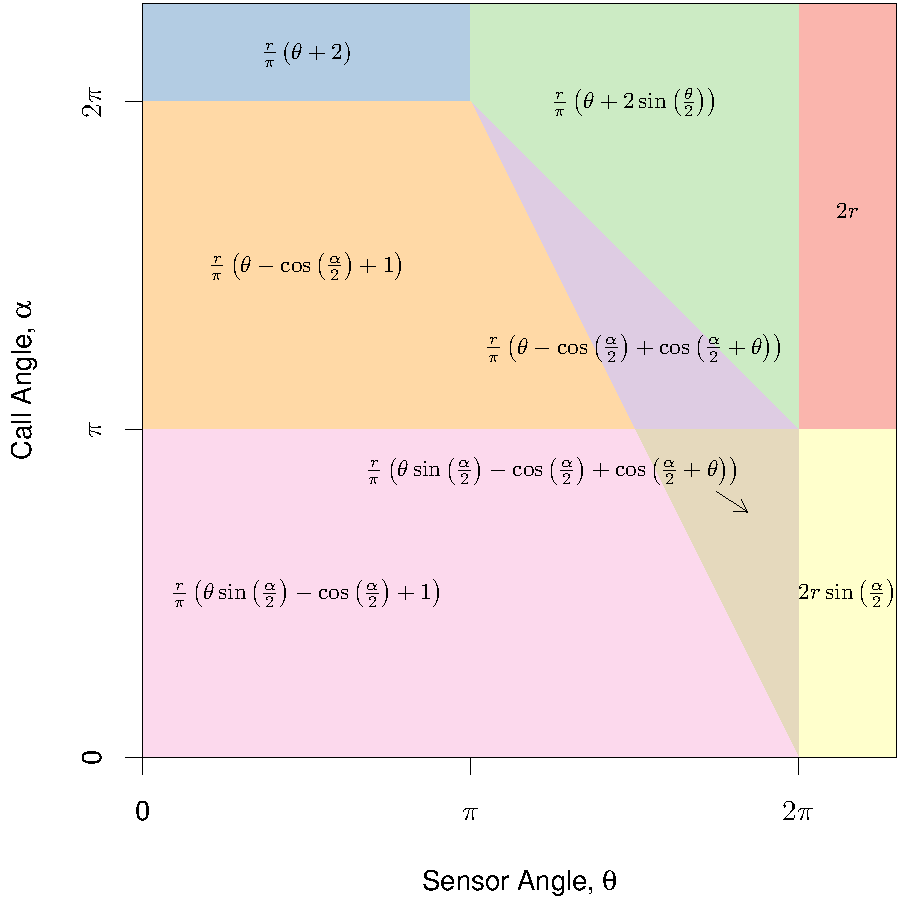
\includegraphics[width=1\textwidth]{imgs/equalModelResults.pdf}
\caption[REM model solutions]{The results of the models grouped so that all the regions with equal results are presented only once.}
\label{f:equalModelResults}
\end{figure}
\end{comment}

\subsubsection{Model SW9} \label{SW9}

Finally, SW9, the last model, is bounded by y $\alpha \le \pi - 2\theta$, $\alpha \ge 2\theta$ and $\theta \ge 0$. Therefore it starts with a $\theta$ limited profile. However it doesn't contain the extra $x_2$ profile nor a $x_4$ profile.

\begin{align}
    \bar{p}_{\text{\tiny{SW9}}} =&\frac{1}{\pi} \left(\;\;\int\limits_{\frac{\pi}{2} - \frac{\theta}{2}}^{\frac{\pi}{2}}2 r \sin{\left (\frac{\theta}{2} \right )} \sin{\left (x_{2} \right )}\;\mathrm{d}x_{2}+\int\limits_{\theta}^{\frac{\alpha}{2}}r \sin{\left (x_{3} \right )}\;\mathrm{d}x_{3}+\int\limits_{\frac{\alpha}{2}}^{\frac{\alpha}{2} + \theta}r \sin{\left (\frac{\alpha}{2} \right )}\;\mathrm{d}x_{3}\right)\label{pSW9Def}\\
    \bar{p}_{\text{\tiny{SW9}}}  =& \frac{r}{\pi} \left(\theta \sin{\left (\frac{\alpha}{2} \right )} - \cos{\left (\frac{\alpha}{2} \right )} + 1\right)\label{pSW9Sln}
\end{align}






